%  !TeX  root  =  user_guide.tex

\chapter{Интеграция с GRASS GIS}\label{sec:grass}\index{GRASS}

% when the revision of a section has been finalized,
% comment out the following line:
%\updatedisclaimer

Расширение GRASS предоставляет доступ к базам данных ГИС GRASS~\cite{GRASSweb}
и ее функциональности, включая визуализацию растровых и векторных слоёв
GRASS, оцифровку векторных слоёв, правку атрибутивных данных,
создание новых векторных слоёв и анализ 2D и 3D данных GRASS с помощью
более чем 300~модулей.

В этом разделе описывается функциональность расширения GRASS и даются
некоторые примеры управления данными GRASS и работы с ними. При запуске
расширения GRASS, как описано в разделе~\ref{sec:starting_grass},
через меню предоставляются следующие функции:

\begin{itemize}[label=--]
\item \toolbtntwo{grass_open_mapset}{Открыть набор}
\item \toolbtntwo{grass_new_mapset}{Новый набор}
\item \toolbtntwo{grass_close_mapset}{Закрыть набор}
\item \toolbtntwo{grass_add_vector}{Добавить векторный слой GRASS}
\item \toolbtntwo{grass_add_raster}{Добавить растровый слой GRASS}
\item \toolbtntwo{grass_new_vector_layer}{Создать новый векторный слой
GRASS}
\item \toolbtntwo{grass_edit}{Редактировать векторный слой GRASS}
\item \toolbtntwo{grass_tools}{Открыть инструменты GRASS}
%\item \toolbtntwo{grass_shell}{Open GRASS Shell}
\item \toolbtntwo{grass_region}{Показать текущий регион GRASS}
\item \toolbtntwo{grass_region_edit}{Изменить текущий регион GRASS}
\end{itemize}

\section{Запуск расширения GRASS}\label{sec:starting_grass}
\index{GRASS!запуск QGIS}

Для использования функциональности GRASS и/или визуализации векторных
и растровых слоёв GRASS в QGIS необходимо выбрать и загрузить расширение
GRASS в Менеджере модулей. Для этого выберите в меню
\mainmenuopt{Модули} \arrow \mainmenuopt{Управление модулями}, выберите
\dropmenuopt{GRASS} и нажмите кнопку \button{OK}.

Теперь вы можете подключать растровые и векторные слои из существующей
\filename{Области} GRASS (см. раздел~\ref{sec:load_grassdata}). Также
вы можете создать новую \filename{Область} GRASS в QGIS (см.
раздел~\ref{sec:create_loc}) и импортировать растровые и векторные
данные (см. раздел~\ref{sec:import_loc_data}) для дальнейшего анализа
с помощью Инструментов GRASS (см. раздел~\ref{subsec:grass_toolbox}).

\section{Загрузка растровых и векторных слоёв GRASS}\label{sec:load_grassdata}\index{GRASS!загрузка данных}

С помощью расширения GRASS вы можете подключать векторные или растровые
слои, используя соответствующую кнопку в панели меню. В качестве примера
мы используем набор данных <<Alaska>> для QGIS (см. раздел~\ref{label_sampledata}).
Он включает небольшую пробную \filename{Область} GRASS с 3~векторными
слоями и 1~растровой картой рельефа.

\begin{enumerate}
  \item Создайте новую папку \filename{grassdata}, загрузите набор
  данных <<Alaska>> \filename{qgis\_sample\_data.zip} по ссылке
  \url{http://download.osgeo.org/qgis/data/} и разархивируйте файл в
  папку \filename{grassdata}.
  \item Запустите QGIS.
  \item Если предыдущая сессия QGIS еще не закончена, подключите
  модуль GRASS: нажмите \mainmenuopt{Модули} \arrow \mainmenuopt{Управление
  модулями} и выберите \dropmenuopt{GRASS}. Должна появиться панель
  GRASS.
  \item В панели GRASS нажмите на иконку
  \toolbtntwo{grass_open_mapset}{Открыть набор} для появления диалога
  с выбором \filename{Набора}.
  \item В графе \filename{Gisdbase} (база данных) выберите или введите
  путь к недавно созданной папке \filename{grassdata}.
  \item Теперь Вы можете выбрать район \filename{alaska} и набор
  \filename{demo}.
  \item Нажмите \button{OK}. Обратите внимание, что некоторые ранее
  недоступные инструменты на панели GRASS теперь доступны.
  \item Нажмите на кнопку \toolbtntwo{grass_add_raster}{Добавить
  растровый слой GRASS}, выберите название слоя \filename{gtopo30}
  и нажмите кнопку \button{OK}. Будет отображена карта рельефа.
  \item Нажмите на кнопку \toolbtntwo{grass_add_vector}{Добавить
  векторный слой GRASS}, выберите название слоя \filename{alaska}
  и нажмите кнопку \button{OK}. Векторный слой границ штата Аляска
  будет наложен поверх слоя \usertext{gtopo30}. Теперь Вы можете
  изменять свойства слоя (прозрачность, параметры заливки, параметры
  обводки и~др.), как описано в главе~\ref{sec:vectorprops}.
  \item Откройте также два других векторных слоя "--- \filename{rivers}
  и \filename{airports} "--- и настройте их свойства.
\end{enumerate}

Как видно, в QGIS очень просто открывать растровые и векторные слои
GRASS. Смотрите соответствующие разделы по редактированию данных GRASS
и созданию новой \filename{Области}. Другие наборы данных GRASS
доступны на сайте \url{http://grass.osgeo.org/download/data.php}.

\begin{Tip}\caption{\textsc{Подключение данных GRASS}}
Если у вас возникли проблемы с подключением данных или QGIS завершает
работу некорректно, убедитесь, что вы правильно включили модуль GRASS,
как описывается в разделе~\ref{sec:starting_grass}.
\end{Tip}

\section{Область и набор GRASS}\label{sec:about_loc}

Данные GRASS находятся в директории, названной GISDBASE. Эта директория
часто именуется \filename{grassdata}, она должна быть создана до того,
как вы начнете работать с модулем GRASS в QGIS. Внутри этой директории
данные GRASS организованы в виде проектов, содержащихся в поддиректориях,
называемых \filename{Область}. Каждая \filename{Область} определяется
ее системой координат, проекцией и географическим охватом. Каждая
\filename{Область} может содержать несколько \filename{Наборов}
(поддиректории \filename{Области}), которые используются для разделения
проекта по различным темам, субрегионам, или в качестве отдельных
наборов для разных членов рабочей группы (Neteler \& Mitasova 2008
\cite{neteler_mitasova08}). Для того, чтобы проводить анализ векторных
и растровых слоев с помощью модулей GRASS, необходимо импортировать их
в \filename{Область} GRASS.
\footnote{Строго говоря, это не совсем так "--- с помощью модулей GRASS
\filename{r.external} и \filename{v.external} можно создавать ссылки
(только для чтения) на внешние GDAL/OGR-совместимые данные без их
импорта. Но т.\,к. это не совсем обычный способ начать работу с GRASS
для новичков, эти функции не будут описаны здесь.}


\begin{figure}[ht]
\centering

\includegraphics[clip=true]{grass_location}
\caption{Данные GRASS в районе <<alaska>> (адаптировано из Neteler \& Mitasova 2008 \cite{neteler_mitasova08})}\label{fig:grass_location}\end{figure}

\subsection{Создание новой области GRASS}\label{sec:create_loc}

В качестве примера вы найдете здесь инструкции, по которым была создана
пробная \filename{Область} <<alaska>> в равновеликой конической проекции
Альберса с единицами измерения в футах. Эта область может быть использована
для всех примеров и упражнений в последующих разделах, связанных с ГИС
GRASS. Так что будет полезно загрузить и установить этот набор данных на ваш
компьютер \ref{label_sampledata}.

\begin{figure}[ht]
\centering
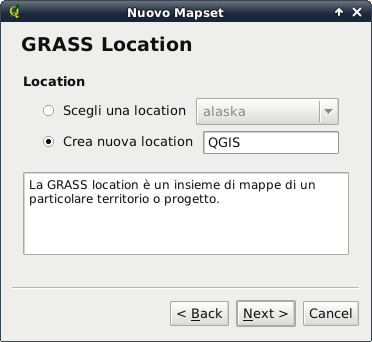
\includegraphics[clip=true, width=8cm]{create_grass_location}
\caption{Создание новой области \grass или нового набора в \qg \wincaption}
\label{fig:create_grass_location}
\end{figure}

\begin{enumerate}
  \item Запустите QGIS и убедитесь, что расширение GRASS загружено.
  \item Откройте shape-файл \filename{alaska.shp} (см. раздел~\ref{sec:load_shapefile}
  из набора данных <<Alaska>>~\ref{label_sampledata}.
  \item На панели GRASS нажмите на кнопку \toolbtntwo{grass_open_mapset}{Открыть набор}
  для появления диалога с выбором \filename{Набора}.
  \item Выберите существующую директорию базы данных GRASS (GISDBASE)
  \filename{grassdata} или создайте таковую для новой \filename{Области},
  используя файловый менеджер. Затем нажмите кнопку \button{Next}.
  \item Можно использовать этот диалог для создания нового \filename{Набора}
  в существующей \filename{Области} (см. раздел~\ref{sec:add_mapset}) или
  для создания новой \filename{Области}. Выберите пункт
  \radiobuttonon{{}Создать новый район} (см. Рисунок~\ref{fig:create_grass_location}).
  \item Введите имя \filename{Области} (мы используем <<alaska>>) и
  нажмите кнопку \button{Next}.
  \item Определите проекцию, выбрав пункт \radiobuttonon{{}Проекция}
  и включив список проекций.
  \item Мы используем равновеликую коническую проекцию Альберса (в футах).
  Когда мы узнали, что она представлена EPSG-кодом 2964, вводим код в
  графу поиска. (Замечание: Если вы хотите повторить этот процесс для
  другого \filename{Региона} и другой проекции, не обязательно запоминать
  код EPSG, просто нажмите значок
  \toolbtntwo{mIconProjectionEnabled}{Преобразование координат}
  в нижнем правом углу статус-бара (см. раздел~\ref{label_projstart}))
  \item Нажмите кнопку \button{Find} для выбора проекции.
  \item Нажмите кнопку \button{Next}.
  \item Чтобы определить регион по умолчанию, мы должны ввести границы
  \filename{Области} в северном, южном, западном и восточном направлении.
  Здесь мы просто нажимаем на кнопку \\
  \button{Установить текущие границы QGIS}, чтобы применить охват
  открытого слоя \filename{alaska.shp} в качестве региона GRASS
  по умолчанию.
  \item Нажмите кнопку \button{Next}.
  \item Также мы должны определить \filename{Набор} внутри нашей
  новой \filename{Области}. Вы можете называть его как угодно "--- мы
  используем имя <<demo>>.
  \footnote{Когда создается новая \filename{Область}, GRASS автоматически
  создает специальный \filename{Набор}, называемый \filename{PERMANENT},
  спроектированный для хранения главных данных проекта, его исходного
  пространственного охвата и определений системы координат
  (Neteler \& Mitasova 2008 \cite{neteler_mitasova08}).}
  \item Проверьте общий вывод, чтобы быть уверенным в корректности
  введенного, и нажмите \button{Finish}.
\item Были созданы: новая \filename{область} \filename{alaska} и два \filename{Набора}~---
    \filename{demo} и \filename{PERMANENT}. Текущий
  рабочий набор "--- \filename{MAPSET demo}, как было задано.
  \item Обратите внимание, что некоторые из инструментов на панели
  GRASS, которые раньше были отключены, теперь доступны.
\end{enumerate}

Хотя все это выглядит как множество ходов, в реальности не все так плохо
и это очень быстрый способ создания \filename{Области}.
\filename{Область alaska} теперь готова для импорта данных (см.
раздел~\ref{sec:import_loc_data}). Вы также можете использовать уже
имеющиеся векторные и растровые данные в \filename{Области alaska},
включенные в набор данных для QGIS <<Alaska>> \ref{label_sampledata} и
перейти к разделу~\ref{label_vectmodel}.

\subsection{Добавление нового набора}\label{sec:add_mapset}

Пользователь имеет права для записи только в тот \filename{Набор}
GRASS, который он создал. Это означает, что, кроме доступа к своему
\filename{Набору}, каждый пользователь имеет права чтения файлов карт в
\filename{Наборах} других пользователей, но он может изменять или
удалять карты только в своем \filename{Наборе}. Все \filename{Наборы}
включают файл \filename{WIND}, который содержит текущие значения
координат и текущее выбранное разрешение растров (Neteler \& Mitasova 2008
\cite{neteler_mitasova08}, см. раздел~\ref{sec:grass_region}).

\begin{enumerate}
  \item Запустите QGIS и убедитесь, что расширение GRASS загружено.
  \item На панели GRASS нажмите кнопку \toolbtntwo{grass_new_mapset}{Новый набор}
  для появления диалога с выбором \filename{Набора}.
  \item Выберите папку базы данных GRASS (GISDBASE) \filename{grassdata}
  с \filename{Областью alaska}, где мы хотим добавить следующий
  \filename{Набор} с именем test.
  \item Нажмите кнопку \button{Next}.
  \item Мы можем использовать этот диалог для создания нового
  \filename{Набора} в существующей \filename{Области}
  (см. раздел~\ref{sec:add_mapset}) или для создания новой
  \filename{Области}. Выберите пункт \radiobuttonon{{}Выбрать район}
  (см. Рисунок~\ref{fig:create_grass_location}) и нажмите кнопку \button{Next}.
  \item Введите имя \filename{test} для нового \filename{Набора}. Ниже
  в диалоге вы видите список имеющихся \filename{Наборов} и их владельцев.
  \item Нажмите кнопку \button{Next}, проверьте общий вывод, чтобы быть
  уверенными в корректности введенного, и нажмите кнопку \button{Finish}.
\end{enumerate}

\section{Импорт данных в область GRASS}\label{sec:import_loc_data}

Этот раздел показывает пример того, как импортируются растровые и
векторные данные в \filename{Область} GRASS \filename{alaska},
представленные в наборе данных QGIS <<Alaska>>. Для этого мы используем
растровую карту растительности \filename{landcover.img} и векторный
GML-файл \filename{lakes.gml} из набора данных QGIS \ref{label_sampledata}.

\begin{enumerate}
  \item Запустите QGIS и убедитесь, что расширение GRASS загружено.
  \item На панели GRASS нажмите кнопку \toolbtntwo{grass_open_mapset}{Открыть набор}
  для появления диалога с выбором \filename{Набора}
  \item Выберите папку базы данных GRASS \filename{grassdata} в наборе
  данных QGIS <<alaska>>, далее \filename{Область alaska} и \filename{Набор}
  \filename{demo}, нажмите кнопку \button{OK}.
  \item Теперь нажмите кнопку \toolbtntwo{grass_tools}{Открыть инструменты GRASS}.
  Появится окно инструментов GRASS (см. раздел~\ref{subsec:grass_toolbox}).
  \item Для импорта растрового слоя \filename{landcover.img}, выберите
  модуль \filename{r.in.gdal} на вкладке \tab{Дерево модулей}. Этот
  модуль GRASS позволяет импортировать растровые файлы, поддерживаемые
  GDAL, в \filename{Область} GRASS. Появится окно модуля \filename{r.in.gdal}.
  \item Откройте папку \filename{raster} в наборе данных QGIS <<alaska>>
  и выберите файл \filename{landcover.img}.
  \item Определите имя выходного растра как \filename{landcover\_grass},
  нажмите кнопку \button{Выполнить}. Во вкладке \tab{Вывод} вы видите
  текущую запущенную команду GRASS \\
  \filename{r.in.gdal -o input=/path/to/landcover.img output=landcover\_grass}.
  \item Когда появится надпись \textbf{Успешное завершение}, нажмите кнопку
  \button{Открыть вывод}. Растровый слой \filename{landcover\_grass}
  теперь импортирован в GRASS и может быть показан в окне карты QGIS.
  \item Для импорта векторного GML файла \filename{lakes.gml} выберите
  модуль \filename{v.in.ogr} на вкладке \tab{Дерево модулей}. Этот модуль
  GRASS позволяет импортировать векторные файлы, поддерживаемые OGR, в
  \filename{Область} GRASS. Появится окно модуля \filename{v.in.ogr}.
  \item Откройте папку \filename{gml} в наборе данных QGIS <<alaska>>
  и выберите файл \filename{lakes.gml} как файл OGR.
  \item Определите имя выходного векторного слоя как \filename{lakes\_grass},
  нажмите кнопку \button{Выполнить}. Вы можете не беспокоиться о других
  опциях в этом примере. Во вкладке \tab{Вывод} вы видите текущую
  запущенную команду GRASS \\
  \filename{v.in.ogr -o dsn=/path/to/lakes.gml output=lakes\_grass}.
  \item Когда будет сказано \textbf{Успешное завершение}, нажмите кнопку
  \button{Открыть вывод}. Векторный слой \filename{lakes\_grass} теперь
  импортирован в GRASS и может быть показан в окне карты QGIS.
\end{enumerate}


\section{Модель векторных данных GRASS}\label{label_vectmodel}\index{GRASS!векторная модель}

Важно понять модель векторных данных GRASS до начала процесса оцифровки.\index{GRASS!оцифровка}
В общем виде, GRASS использует топологическую векторную модель.\index{GRASS!топология}
Это означает, что площадные объекты представлены не замкнутыми
полигонами, а одной или более границами. Граница между двумя смежными
полигонами оцифровывается только один раз и является общей для обоих
полигонов. Границы должны быть соединены без разрывов. Полигон
определяется с помощью центроида внутри полигона.

Кроме границ и центроидов, векторный слой содержит также точки и линии.
Все эти геометрические элементы могут быть смешаны в одной векторной
карте, а могут быть представлены в виде так называемых <<слоев>> в
векторной карте GRASS. Таким образом, в GRASS <<слой>> "--- это не
векторная или растровая карта, а <<уровень>> внутри векторной карты.
Важно тщательно разделять эти понятия.
\footnote{Хотя и возможно совмещать геометрические элементы, обычно это
не принято и используется в GRASS только в специальных целях для сетевого
векторного анализа. В большинстве случаев предпочтительнее хранить разные
геометрические элементы в разных слоях.}

Один векторный <<набор>> может содержать больше <<слоёв>>. Например,
поля, леса и озера могут быть помещены в один векторный слой. Смежные
леса и озера могут иметь одну и ту же границу, но они имеют отдельные
аттрибутивные таблицы. Также возможно присоединять аттрибуты к границам.
Например, если граница между озером и лесом "--- дорога, то она имеет
свою таблицу аттрибутов.

<<Слой>> объекта определяется <<слоем>> внутри GRASS. <<Слой>> "--- это
номер, который отражает присутствие более чем одного слоя в наборе
данных (относится ли геометрия к лесу или к озеру?). На сегодняшний день
он может быть только числом, в будущем GRASS будет поддерживать также
названия в виде полей в графическом интерфейсе.

Аттрибуты могут содержаться внутри \filename{Области} GRASS (как DBase
или SQLite) или во внешних таблицах баз данных, например, PostgreSQL,
MySQL, Oracle и т.\,д.\index{GRASS!хранение атрибутов}

Аттрибуты в таблицах баз данных соотносятся с геометрическими
элементами с помощью значения <<категорий>>.\index{GRASS!связь с атрибутами}
<<Категории>> (ключ, ID "--- это целые числа, присоединенные к
геометрическим элементам, они используются как ссылка на ключевую
колонку в базе данных.

\begin{Tip}\caption{\textsc{Изучение модели векторных данных GRASS}}
Лучший способ изучить модель векторных данных GRASS и ее возможности "---
скачать одно из пособий по GRASS, где модель векторных данных описана
более подробно. Смотрите \url{http://grass.osgeo.org/gdp/manuals.php}
для более подробной информации, книг и пособий на нескольких языках.
\end{Tip}

\section{Создание нового векторного слоя GRASS}\label{sec:creating_new_grass_vectors}\index{GRASS!создание нового вектроного слоя|\see{редактирование!создание нового слоя}}

Чтобы создать новый векторный слой GRASS с помощью расширения GRASS,
нажмите значок \\
\toolbtntwo{grass_new_vector_layer}{Создать новый векторный слой GRASS}.
Введите имя в текстовое окно, и можете начать оцифровывать точки, линии
и полигоны, следуя процедуре, описанной в разделе~\ref{grass_digitising}.

В GRASS возможно создание всех геометрических типов объектов (точек,
линий и полигонов) в одном слое, потому что GRASS использует
топологическую векторную модель, так что вам не надо выбирать тип
геометрии, когда создаете новый векторный слой GRASS. Это отличается от
создания shape-файлов в QGIS, т.\,к. они используют векторную модель
<<Simple Feature>> (см. раздел~\ref{sec:create shape}).

\begin{Tip}\caption{\textsc{Создание таблицы атрибутов для нового векторного слоя GRASS}}
Если вы хотите назначить атрибуты оцифрованным геометрическим объектам,
убедитесь, что до начала оцифровки была создана таблица атрибутов с полями.
(см. рисунок~\ref{fig:grass_digitizing_table}).
\end{Tip}

\section{Оцифровка и правка векторных слоёв GRASS}\index{GRASS!инструменты оцифровки}\label{grass_digitising}

Средства оцифровки векторных слоёв GRASS доступны через кнопку \\
\toolbtntwo{grass_edit}{Редактировать векторный слой GRASS} на панели.
Убедитесь, что векторный слой подгружен и он является выбранным слоем в
легенде до того, как использовать инструменты правки.
Рисунок~\ref{fig:grass_digitizing_category} показывает диалог правки
слоя GRASS, появляющийся при нажатии на кнопку редактирования.
Инструменты и настройки обсуждаются в следующих разделах.

\begin{Tip}\caption{\textsc{Оцифровка полигонов в GRASS}}
Если вы хотите создать полигон в GRASS, необходимо вначале оцифровать
границу полигона, задав режим \usertext{Без категорий}. Затем
добавляется центроид (именованная точка) внутрь замкнутой границы в
режиме \usertext{Следующая не используемая}. Причина в том, что
топологическая векторная модель соотносит аттрибутивную информацию
всегда с центроидом, а не с границей.
\end{Tip}

\minisec{Панель инструментов}\label{label_grasstoolbar}

На рисунке~\ref{fig:grass_digitizing_toolbar} показаны инструменты
оцифровки, предоставляемые модулем GRASS. Таблица~\ref{tab:grass_tools}
объясняет их возможные функции.

\begin{figure}[h]
   \centering
   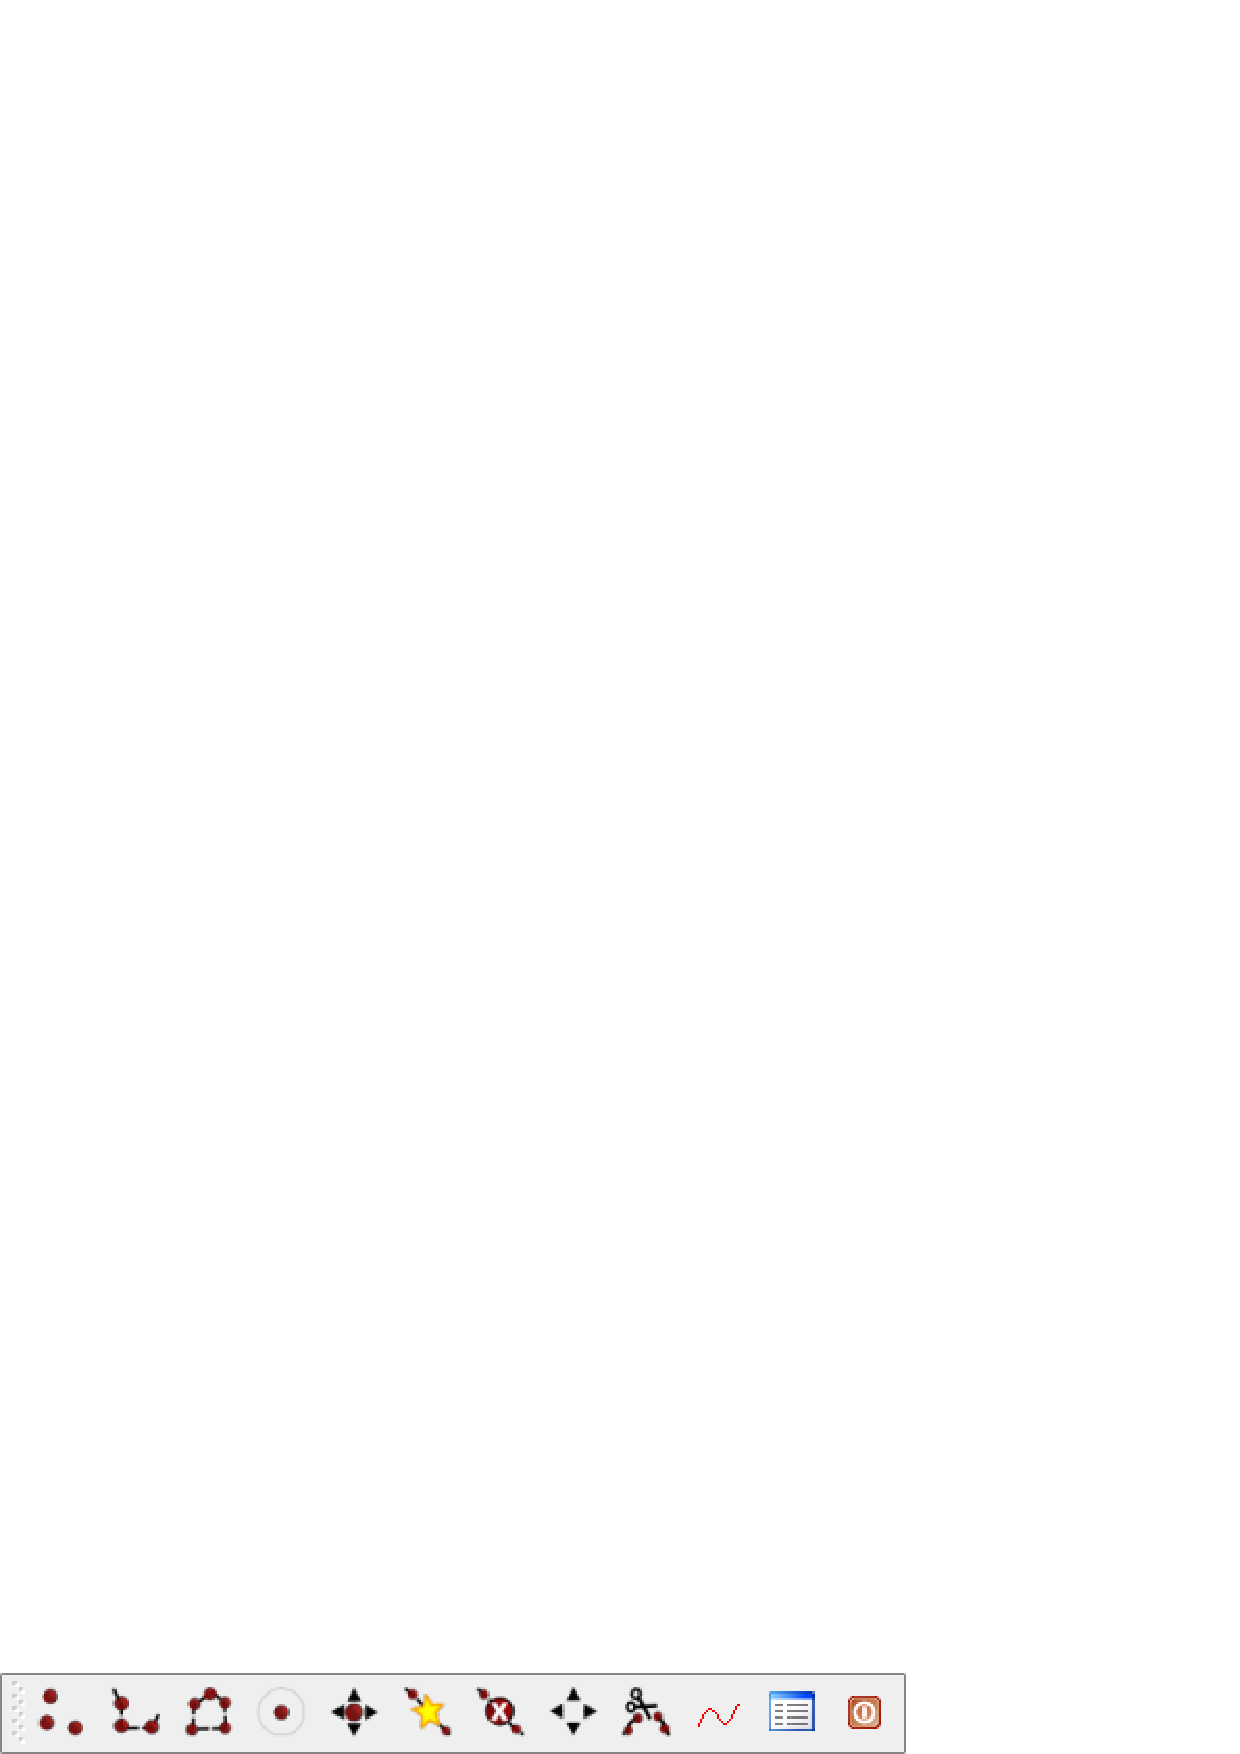
\includegraphics[clip=true,width=12cm]{grass_digitizing_toolbar}
   \caption{Панель инструментов оцифровки GRASS \wincaption}\label{fig:grass_digitizing_toolbar}
\end{figure}

{\renewcommand{\arraystretch}{2}
\begin{table}[h]\index{GRASS!инструменты оцифровки}
\centering
 \begin{tabular}{|m{1cm}|m{4cm}|m{8.5cm}|}
 \hline \textbf{Icon} & \textbf{Tool} & \textbf{Purpose} \\
\hline 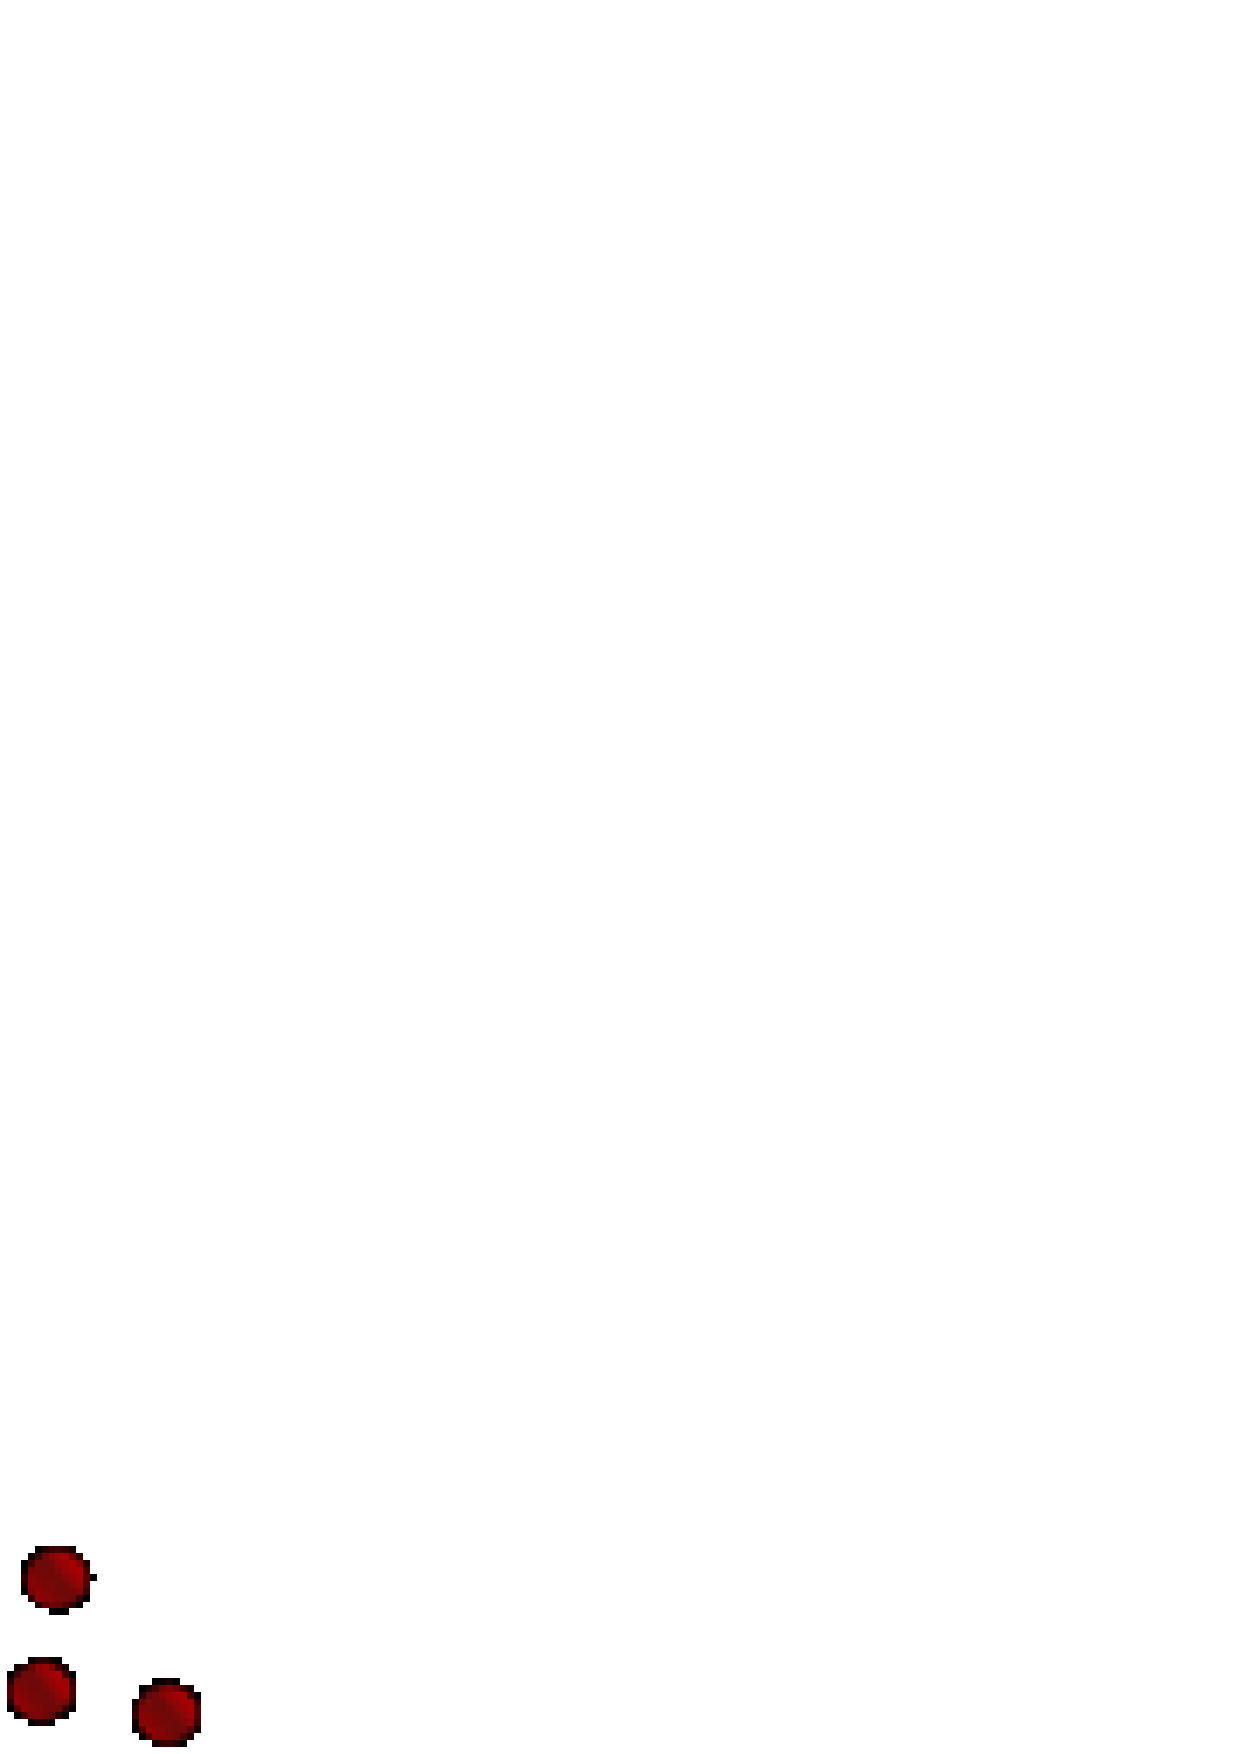
\includegraphics[width=0.7cm]{grass_new_point} & Новая точка &
Оцифровать новую точку \\
\hline 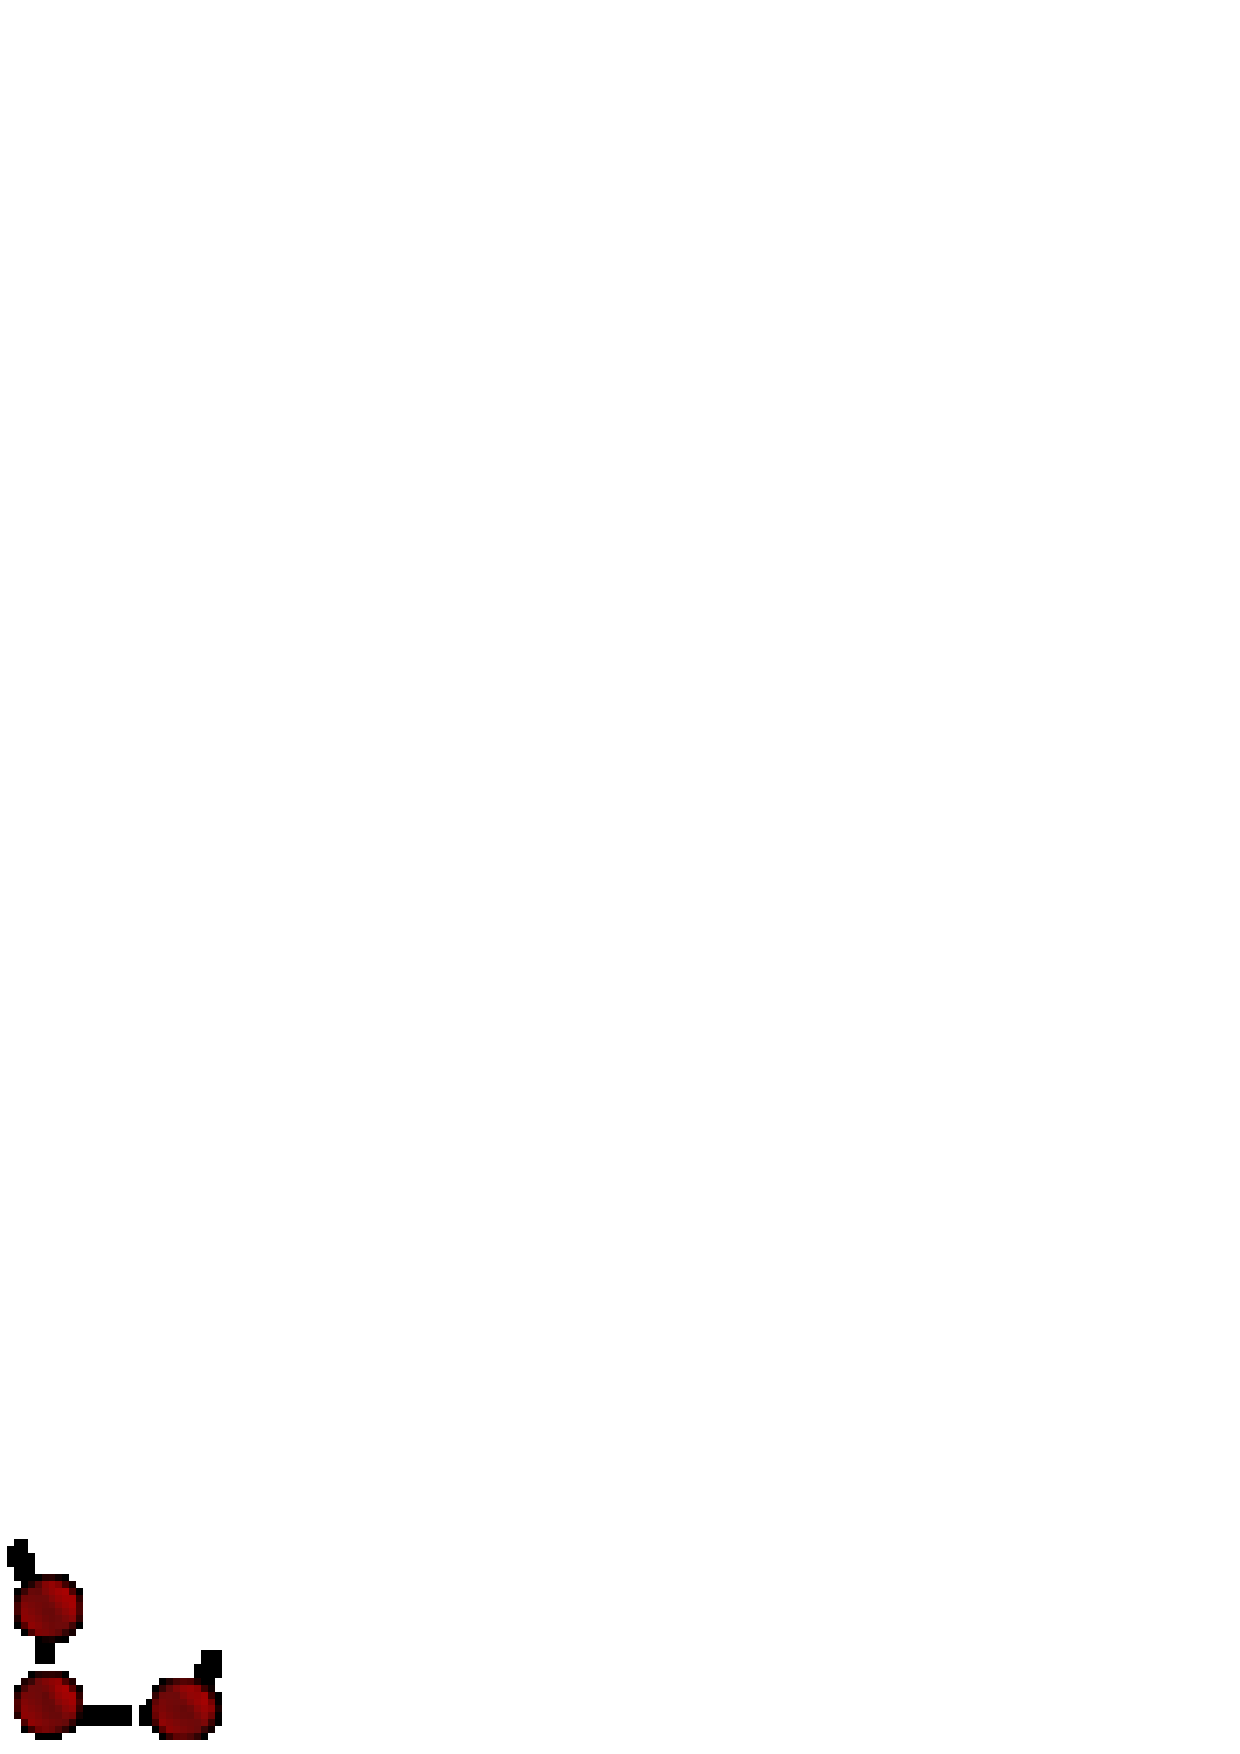
\includegraphics[width=0.7cm]{grass_new_line} & Новая линия &
Оцифровать новую линию (завершается выбором нового инструмента) \\
\hline 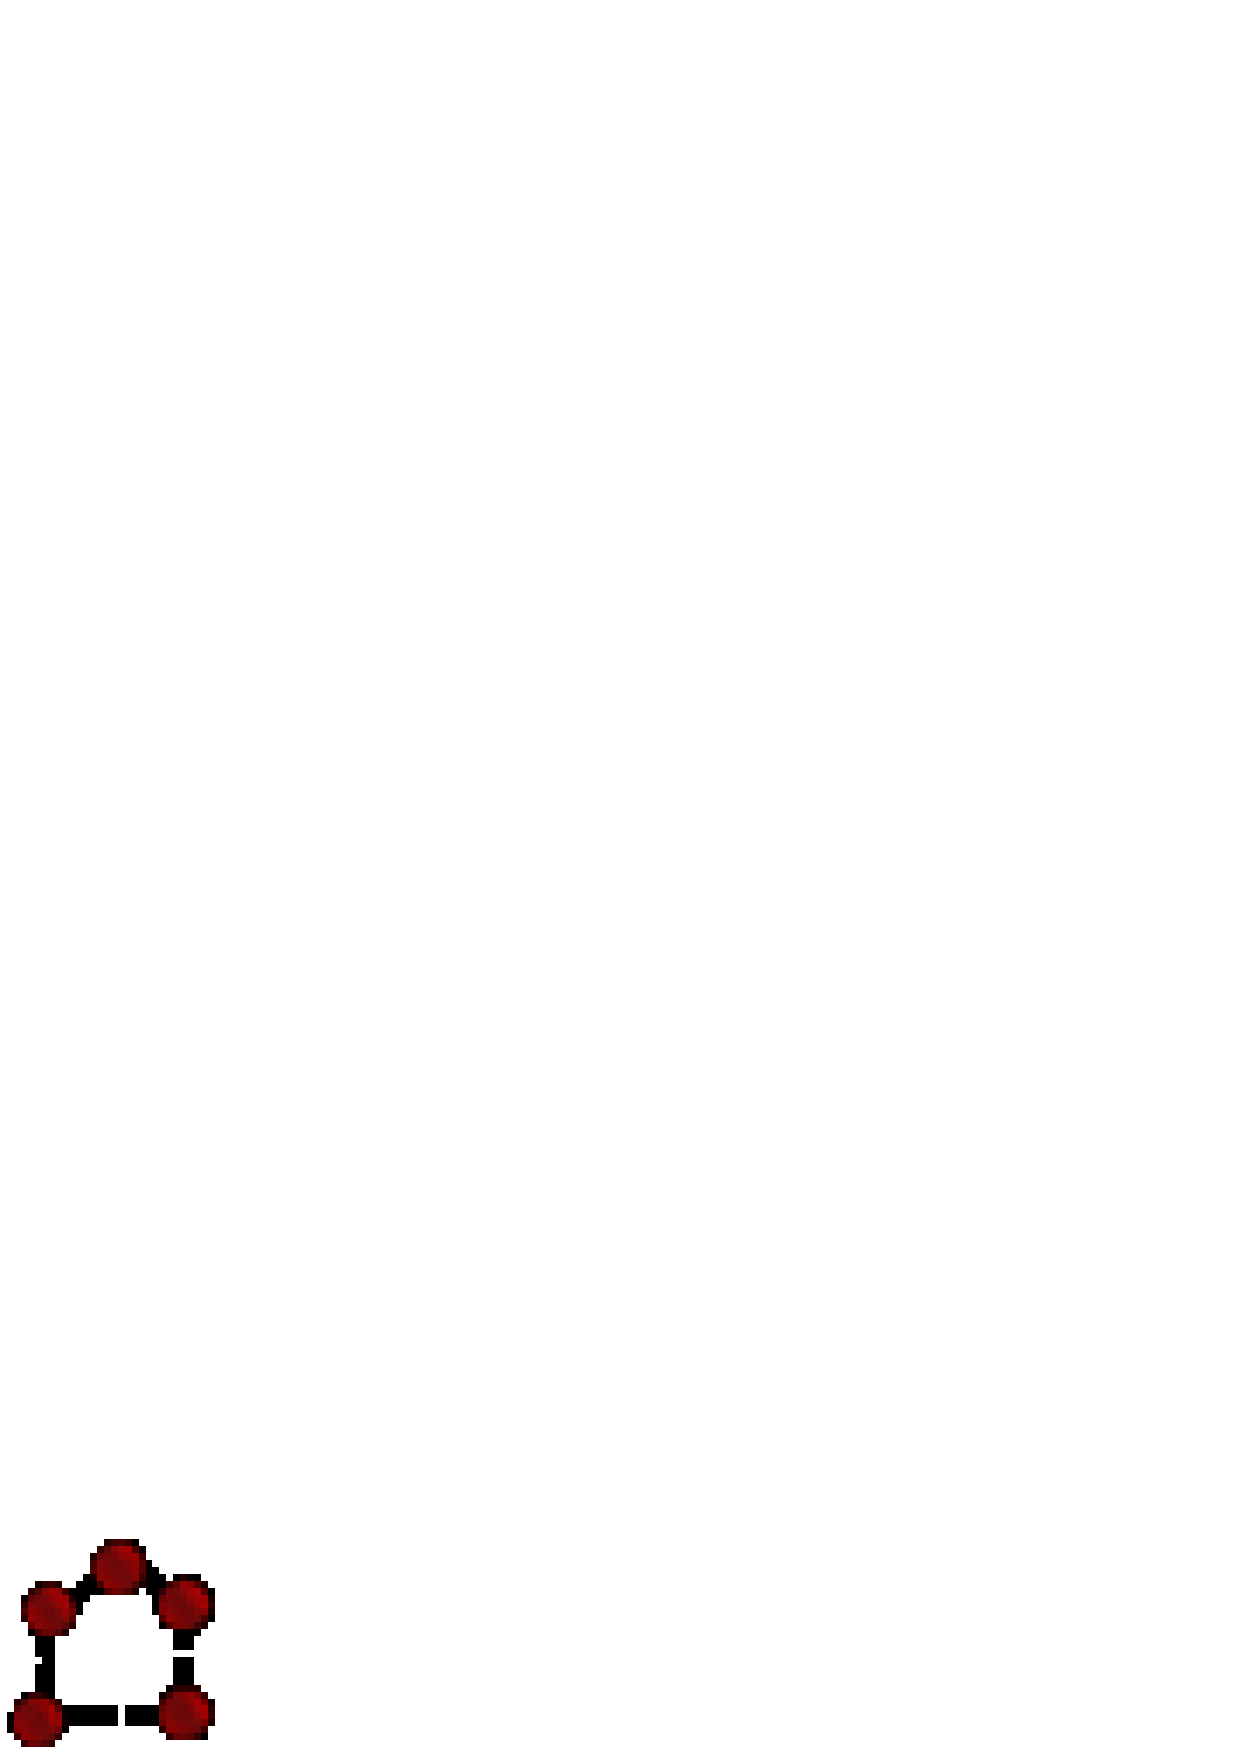
\includegraphics[width=0.7cm]{grass_new_boundary} & Новая граница &
Оцифровать новую границу (завершается выбором нового инструмента) \\
\hline 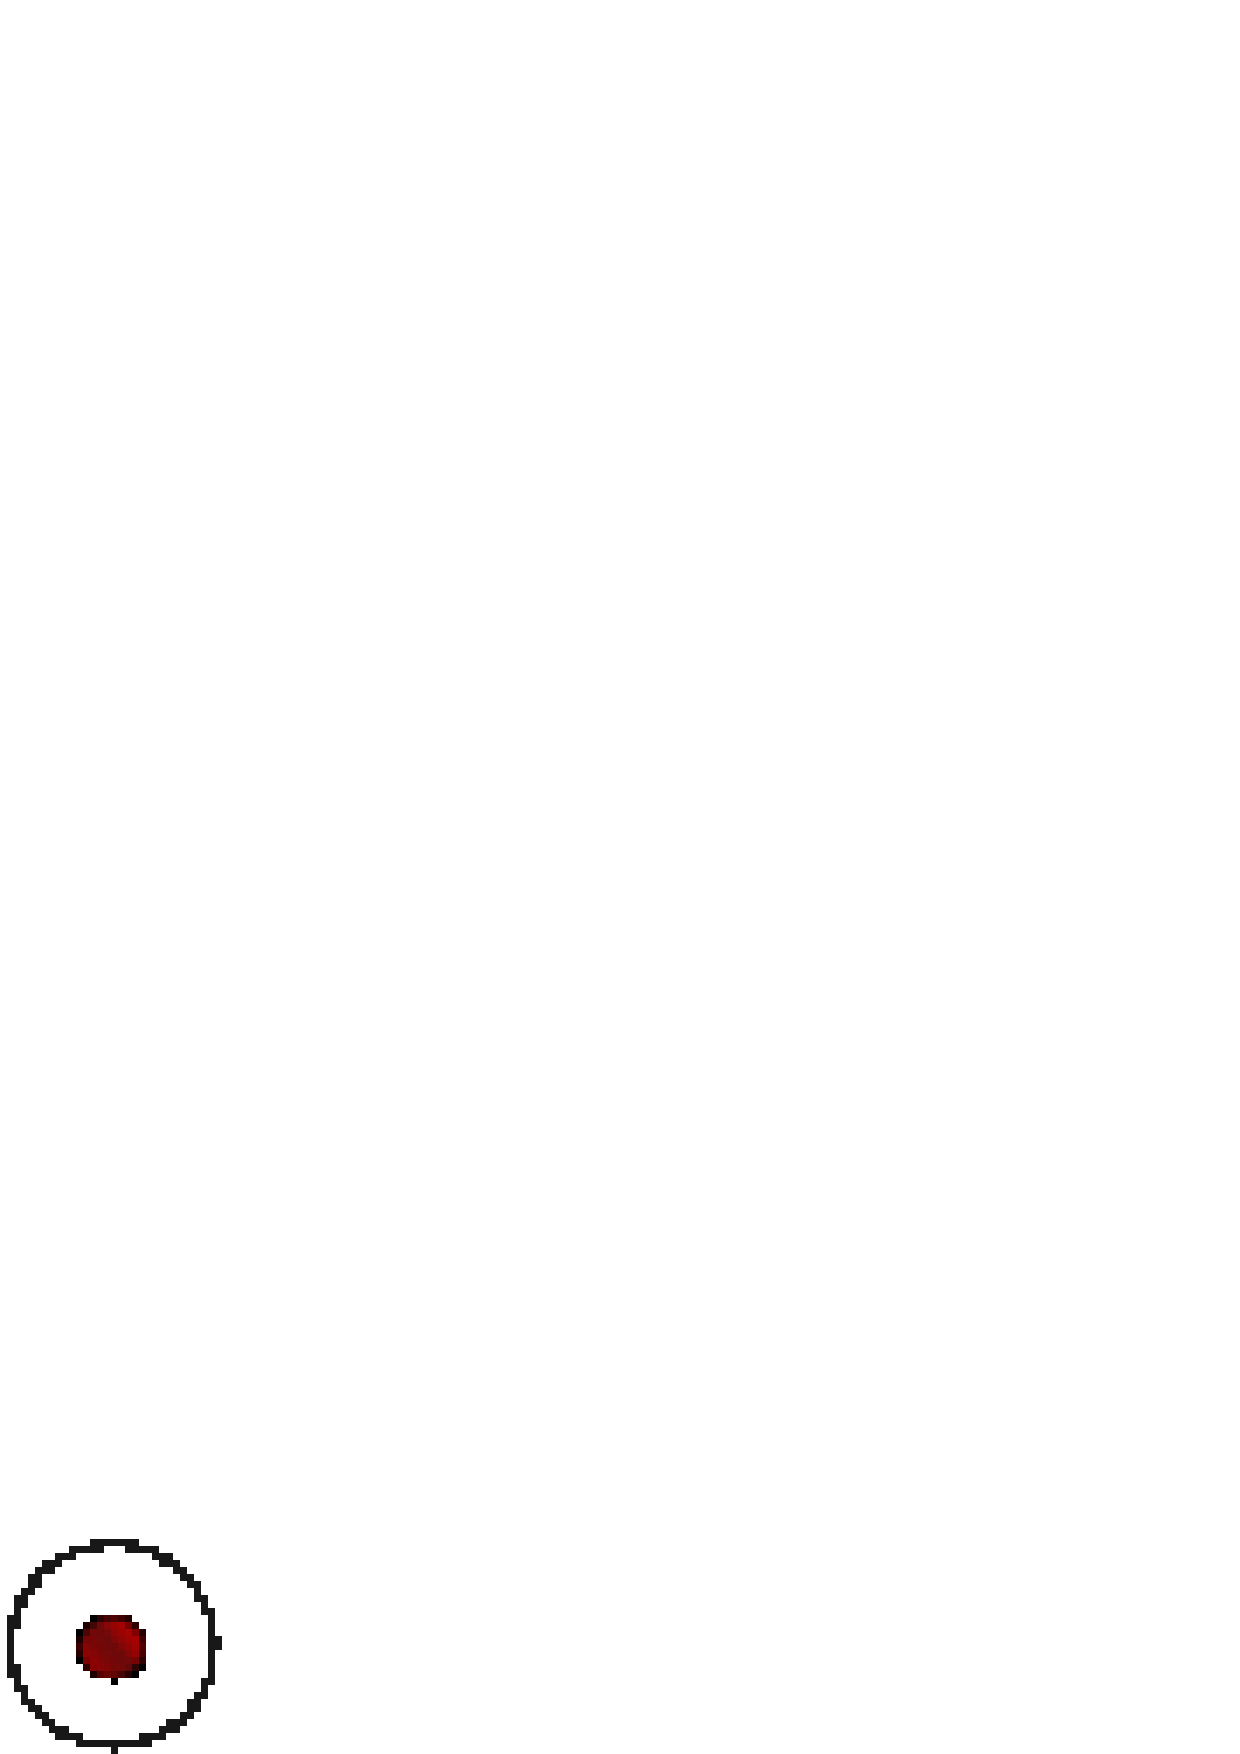
\includegraphics[width=0.7cm]{grass_new_centroid} & New Centroid &
Оцифровать новый центроид (дать метку существующему полигону)\\
\hline 
\includegraphics[width=0.7cm]{grass_move_vertex} & Переместить
вершину & Переместить одну вершину имеющейся линии или границы и
определить новое положение \\
\hline 
\includegraphics[width=0.7cm]{grass_add_vertex} & Добавить
вершину & Добавить новую вершину к существующей линии \\
\hline 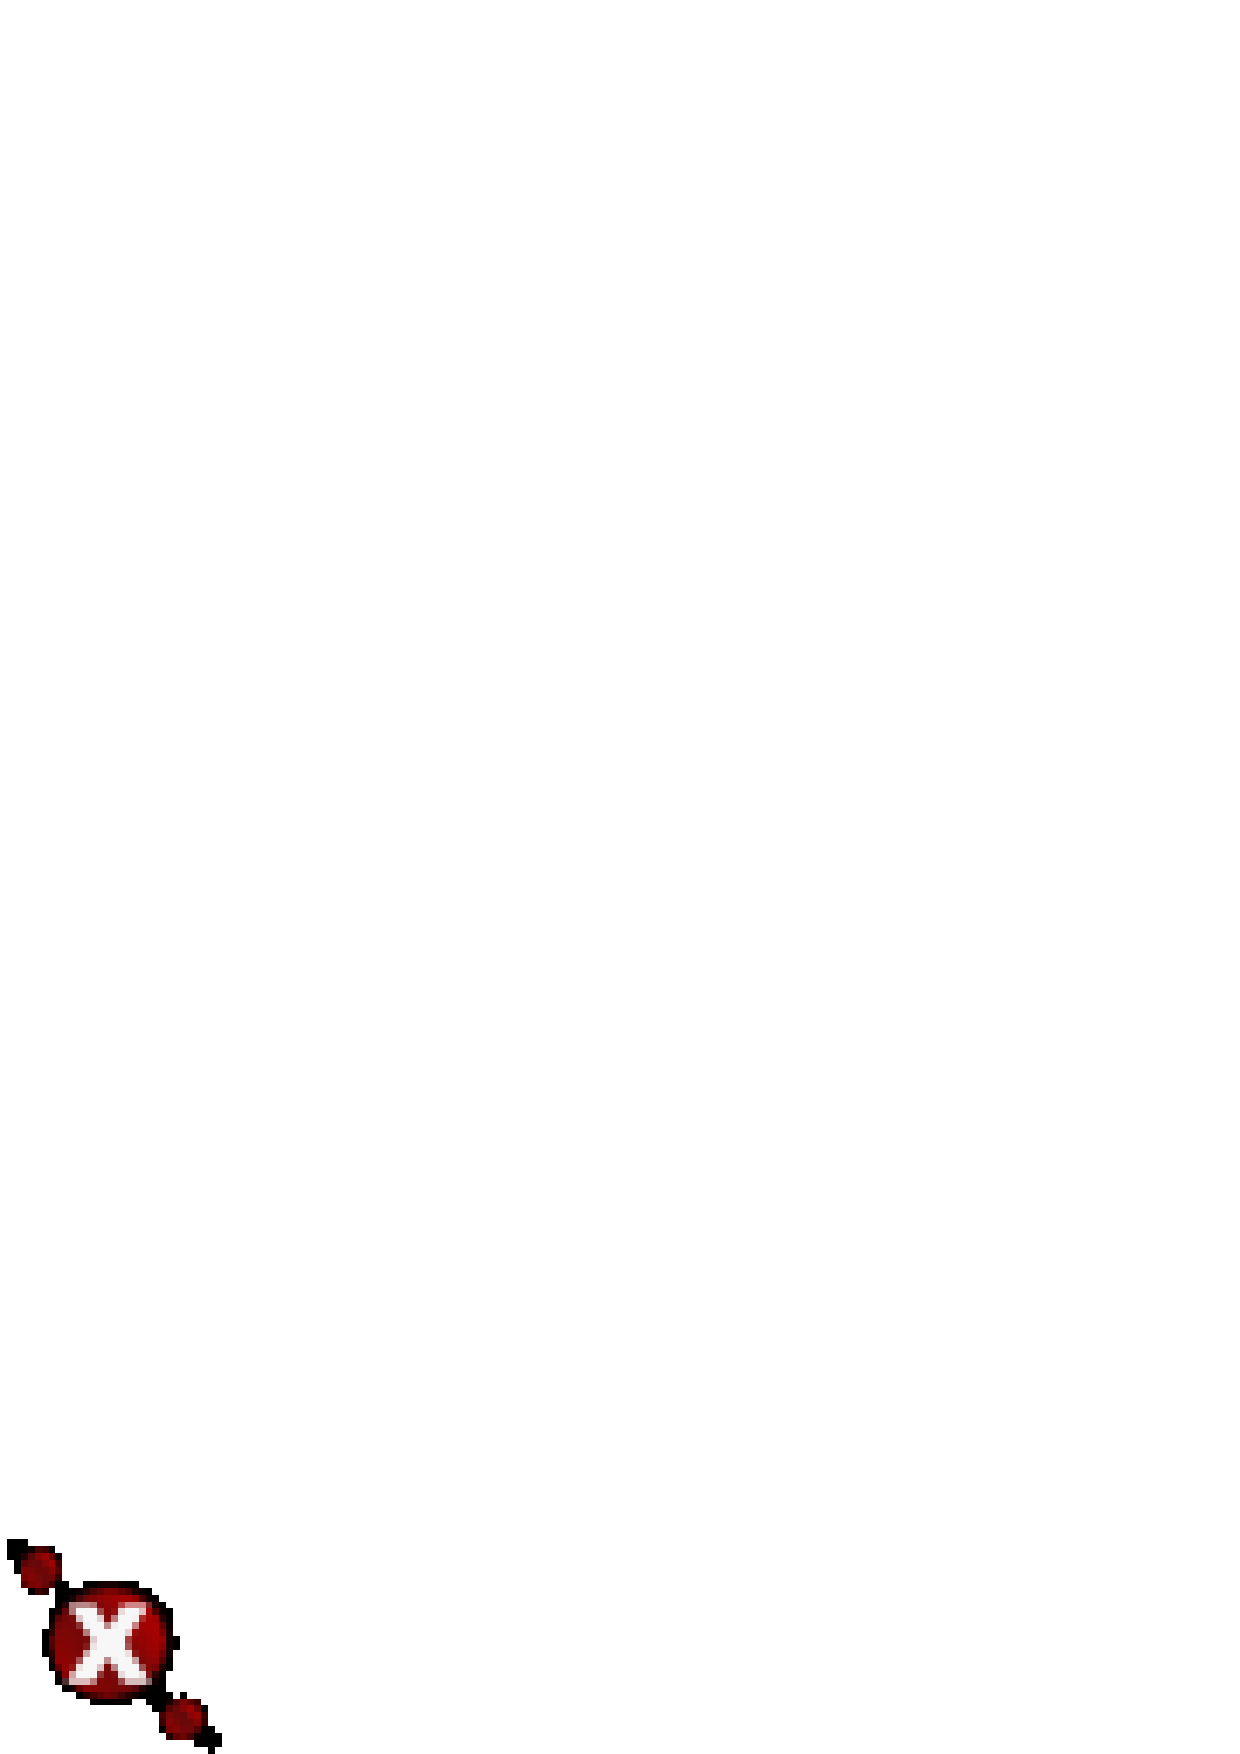
\includegraphics[width=0.7cm]{grass_delete_vertex} & Удалить вершину &
Удалить вершину из существующей линии (подтвердить выбор вершины еще
одним нажатием) \\
\hline 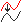
\includegraphics[width=0.7cm]{grass_move_line} & Переместить
элемент & Переместить выбранную границу, линию, точку или центроид
на новую позицию и кликнуть в месте нового положения \\
\hline 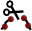
\includegraphics[width=0.7cm]{grass_split_line} & Разбить линию
& Разбить существующую линию на 2~части \\
\hline 
\includegraphics[width=0.7cm]{grass_delete_line} & Удалить элемент &
Удалить существующую границу, линию, точку или центроид (подтвердить выбор элемента еще
одним нажатием) \\
\hline 
\includegraphics[width=0.7cm]{grass_edit_attributes} & Изменить аттрибуты
& Изменить аттрибуты выбранного элемента (заметьте, что один элемент
может представлять много объектов, см.~выше) \\
\hline 
\includegraphics[width=0.7cm]{grass_close_edit} & Закрыть &
Завершить сессию и сохранить текущий статус (с последующей
перестройкой топологии) \\
\hline
\end{tabular}
\caption{Средства оцифровки GRASS}\label{tab:grass_tools}
\end{table}}

\minisec{Вкладка Категории}\index{GRASS!настройка категорий}

Вкладка \tab{Категории} позволяет определить способ присваивания
значений категорий новым геометрическим элементам.

\begin{figure}[h]
 \centering
  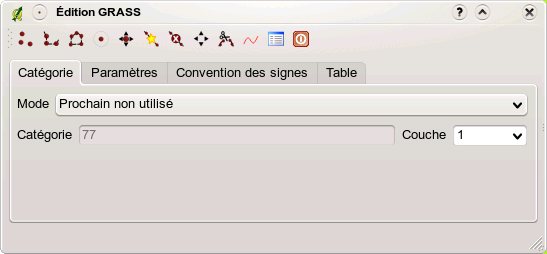
\includegraphics[clip=true,width=8cm]{grass_digitizing_category}
  \caption{Вкладка Категории в панели оцифровки GRASS \wincaption}\label{fig:grass_digitizing_category}
 \end{figure}

\begin{itemize}[label=--]
\item \textbf{Режим}: какое значение категорий должно быть применено к
новым геометрическим элементам.
\begin{itemize}[label=--]
\item Следующая неиспользуемая "--- применяет следующее еще не
использованное значение категорий к геометрическому элементу
\item Ручной ввод "--- значение категорий определяется вручную в
поле <<Категории>>
\item Без категории "--- не применяет значения категорий к
геометрическому элементу. Это используется прежде всего для границ
полигонов, т.\,к. значения категорий присоединяются через центроид.
\end{itemize}
\item \textbf{Категории} "--- Номер (ID), назначенный каждому
оцифрованному геометрическому элементу. Используется для соединения
геометрического элемента с его атрибутами.
\item \textbf{Слой} "--- Каждый геометрический элемент может быть
связан с несколькими атрибутивными таблицами с помощью разных
геометрических слоев GRASS. Номер по умолчанию "--- 1.
\end{itemize}

\begin{Tip}\caption{\textsc{Создание дополнительного <<слоя>> GRASS в QGIS.}}
Если вы хотите добавить больше слоёв в набор данных, просто введите
новый номер в графу <<Слой>> и нажмите Enter. На вкладке \tab{Таблица}
вы можете создать новую таблицу, присоединенную к новому слою.
\end{Tip}

\minisec{Вкладка Параметры}\label{label_settingtab}\index{GRASS!порог прилипания}

Вкладка \tab{Параметры} позволяет задавать прилипание в пикселах
экрана. Порог прилипания определяется тем, на каком расстоянии новые
точки или конечные узлы линий должны быть <<притянуты>> к существующим
узлам. Это помогает избегать разрывов и висячих узлов между
границами. По умолчанию задан порог в 10~пикселов.

\begin{figure}[h]
 \centering
 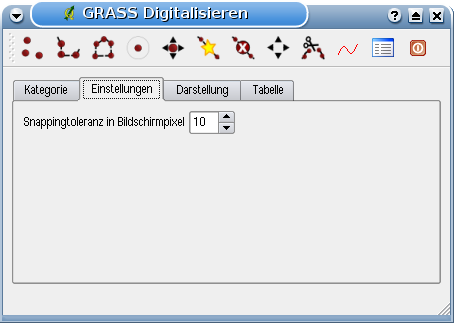
\includegraphics[clip=true,width=8cm]{grass_digitizing_settings}
 \caption{Вкладка Параметры в панели оцифровки GRASS \wincaption}\label{fig:grass_digitizing_settings}
\end{figure}

\minisec{Вкладка Символика}\index{GRASS!настройка символики}

Вкладка \tab{Символика} позволяет просматривать и задавать параметры
символики и цвета для различных геометрических типов и их
топологического статуса (например, закрытая/открытая граница).

\begin{figure}[h]
 \centering
 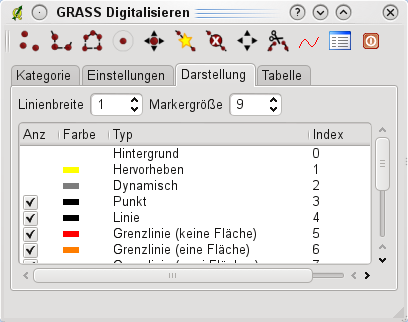
\includegraphics[clip=true,width=8cm]{grass_digitizing_symbology}
 \caption{Вкладка Символика в панели оцифровки GRASS \wincaption}\label{fig:grass_digitizing_symbology}
\end{figure}

\minisec{Вкладка Таблица} \index{GRASS!редактирование таблиц}
Вкладка \tab{Таблица} предоставляет информацию о таблице в базе данных
для данного <<слоя>>. Здесь можно добавить новые поля к существующей
таблице аттрибутов или создать новую таблицу для векторного слоя GRASS
(см. раздел~\ref{sec:creating_new_grass_vectors}).

\begin{figure}[h]
 \centering
 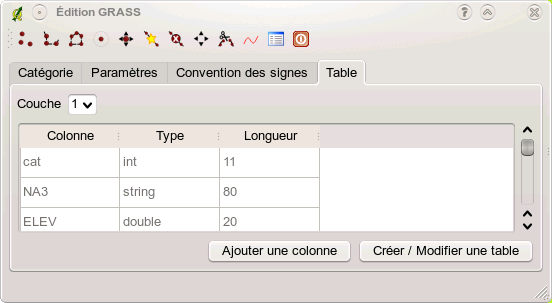
\includegraphics[clip=true,width=10cm]{grass_digitizing_table}
 \caption{Вкладка Таблица в панели оцифровки GRASS \wincaption}\label{fig:grass_digitizing_table}
 \end{figure}

\begin{Tip}\caption{\textsc{Права редактирования GRASS}}\index{GRASS!права редактирования}
Вы должны быть владельцем \filename{Набора} GRASS, данные которого вы
хотите редактировать. Возможно править данные в \filename{Наборе},
который не принадлежит вам, если у вас есть права для записи.
\end{Tip}

\section{Инструмент работы с регионом GRASS}\label{sec:grass_region}\index{GRASS!регион}

Определение региона (задание пространственных характеристик) в GRASS
важно для работы с растровыми данными. Векторный анализ по умолчанию не
ограничен любыми определенными параметрами района. Но все вновь
созданные растры будут иметь пространственный охват и разрешение
текущего региона GRASS (независимо от их оригинального охвата и
разрешения). Текущий регион GRASS находится в файле
\filename{\$LOCATION/\$MAPSET/WIND} и определяет северную, южную,
восточную и западную границы, число столбцов и строк, горизонтальное и
вертикальное пространственное разрешение.

Возможно отключать/включать показ региона GRASS в окне карты QGIS с
помощью кнопки \\
\toolbtntwo{grass_region}{Показать текущий регион GRASS}.\index{GRASS!регион!показ}

С помощью кнопки \toolbtntwo{grass_region_edit}{Изменить текущий регион GRASS}
можно открыть диалог для изменения текущего региона и символики границ
региона в окне QGIS. Наберите новые значения границ и разрешения региона
и нажмите кнопку \button{OK}. Также можно выбрать новый регион
интерактивно с помощью мыши в окне QGIS. Для этого нажмите левой кнопкой
мыши в окне карты QGIS, начните рисовать прямоугольник, закончите также
левой кнопкой и нажмите \button{OK}.\index{GRASS!регион!редактирование}
Модуль GRASS \filename{g.region} предоставляет гораздо больше
параметров для определения необходимого охвата и разрешения для
растрового анализа. Вы можете использовать эти параметры с помощью
модуля инструментов GRASS, описанного в разделе~\ref{subsec:grass_toolbox}.

\section{Панель инструментов GRASS}\label{subsec:grass_toolbox}\index{GRASS!панель инструментов}

Окно \toolbtntwo{grass_tools}{Открыть инструменты GRASS} предоставляет
функциональность модулей GRASS для работы с данными внутри выбранной
\filename{Области} и \filename{Набора}. Чтобы использовать инструменты
GRASS, требуется открыть \filename{Область} и \filename{Набор}, где у
вас есть права записи (обычно даются при создании \filename{Набора}).
Это необходимо, т.\,к. новые растровые и векторные слои, создающиеся в
процессе анализа, должны быть записаны в текущие выбранные
\filename{Область} и \filename{Набор}.

\subsection{Работа с модулями GRASS}\label{grass_modules}\index{GRASS!панель инструментов}

\begin{figure}[ht]
\centering
   \subfloat[Дерево модулей] {\label{subfig:grass_module_tree}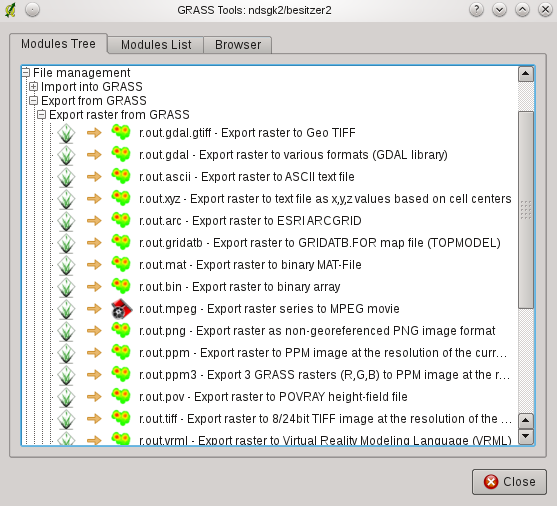
\includegraphics[clip=true, width=0.4\textwidth]{grass_toolbox_moduletree}}
   \hspace{0.5cm}
   \subfloat[Список модулей (с возможностью поиска)] {\label{subfig:grass_module_list}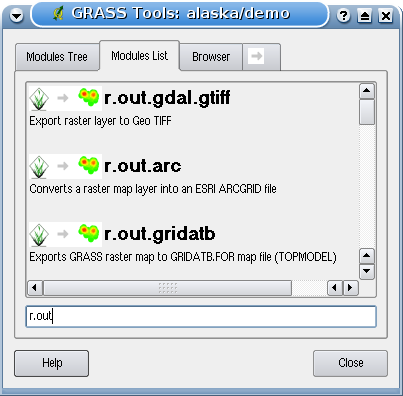
\includegraphics[clip=true, width=0.4\textwidth]{grass_toolbox_modulelist}}
\caption{Инструменты GRASS и поиск по списку модулей \wincaption}\label{fig:grass_modules}
\end{figure}

Оболочка GRASS в панели инструментов предоставляет доступ почти ко всем
(более, чем к 300) модулям GRASS в режиме командной строки. Чтобы
предложить более дружественную по отношению к пользователю рабочую среду,
примерно 200 из числа доступных модулей и их функций представлены также
в графических диалогах. Эти диалоги сгруппированы в категории, также
доступен поиск по ним. Вы можете найти полный список модулей
GRASS, доступных в версии QGIS \CURRENT, в
Приложении~\ref{appdx_grass_toolbox_modules}. Также возможно настраивать
содержимое Инструментов GRASS. Это описано в
разделе~\ref{sec:toolbox-customizing}.

Как показано на рисунке~\ref{fig:grass_modules}, вы можете найти
необходимый модуль GRASS, используя тематически сгруппированный
перечень на вкладке \tab{Дерево модулей} или вкладку \tab{Список модулей}
с возможностью поиска.

Нажатие на графическую иконку модуля открывает новую вкладку, которая
добавляется к диалогу и имеет три собственные вкладки \tab{Параметры},
\tab{Вывод} и \tab{Справка}. На рисунке~\ref{fig:grass_module_dialog}
показан пример модуля \filename{v.buffer}.

\begin{figure}[h]
\centering
   \subfloat[Модули Параметры] {\label{subfig:grass_module_option}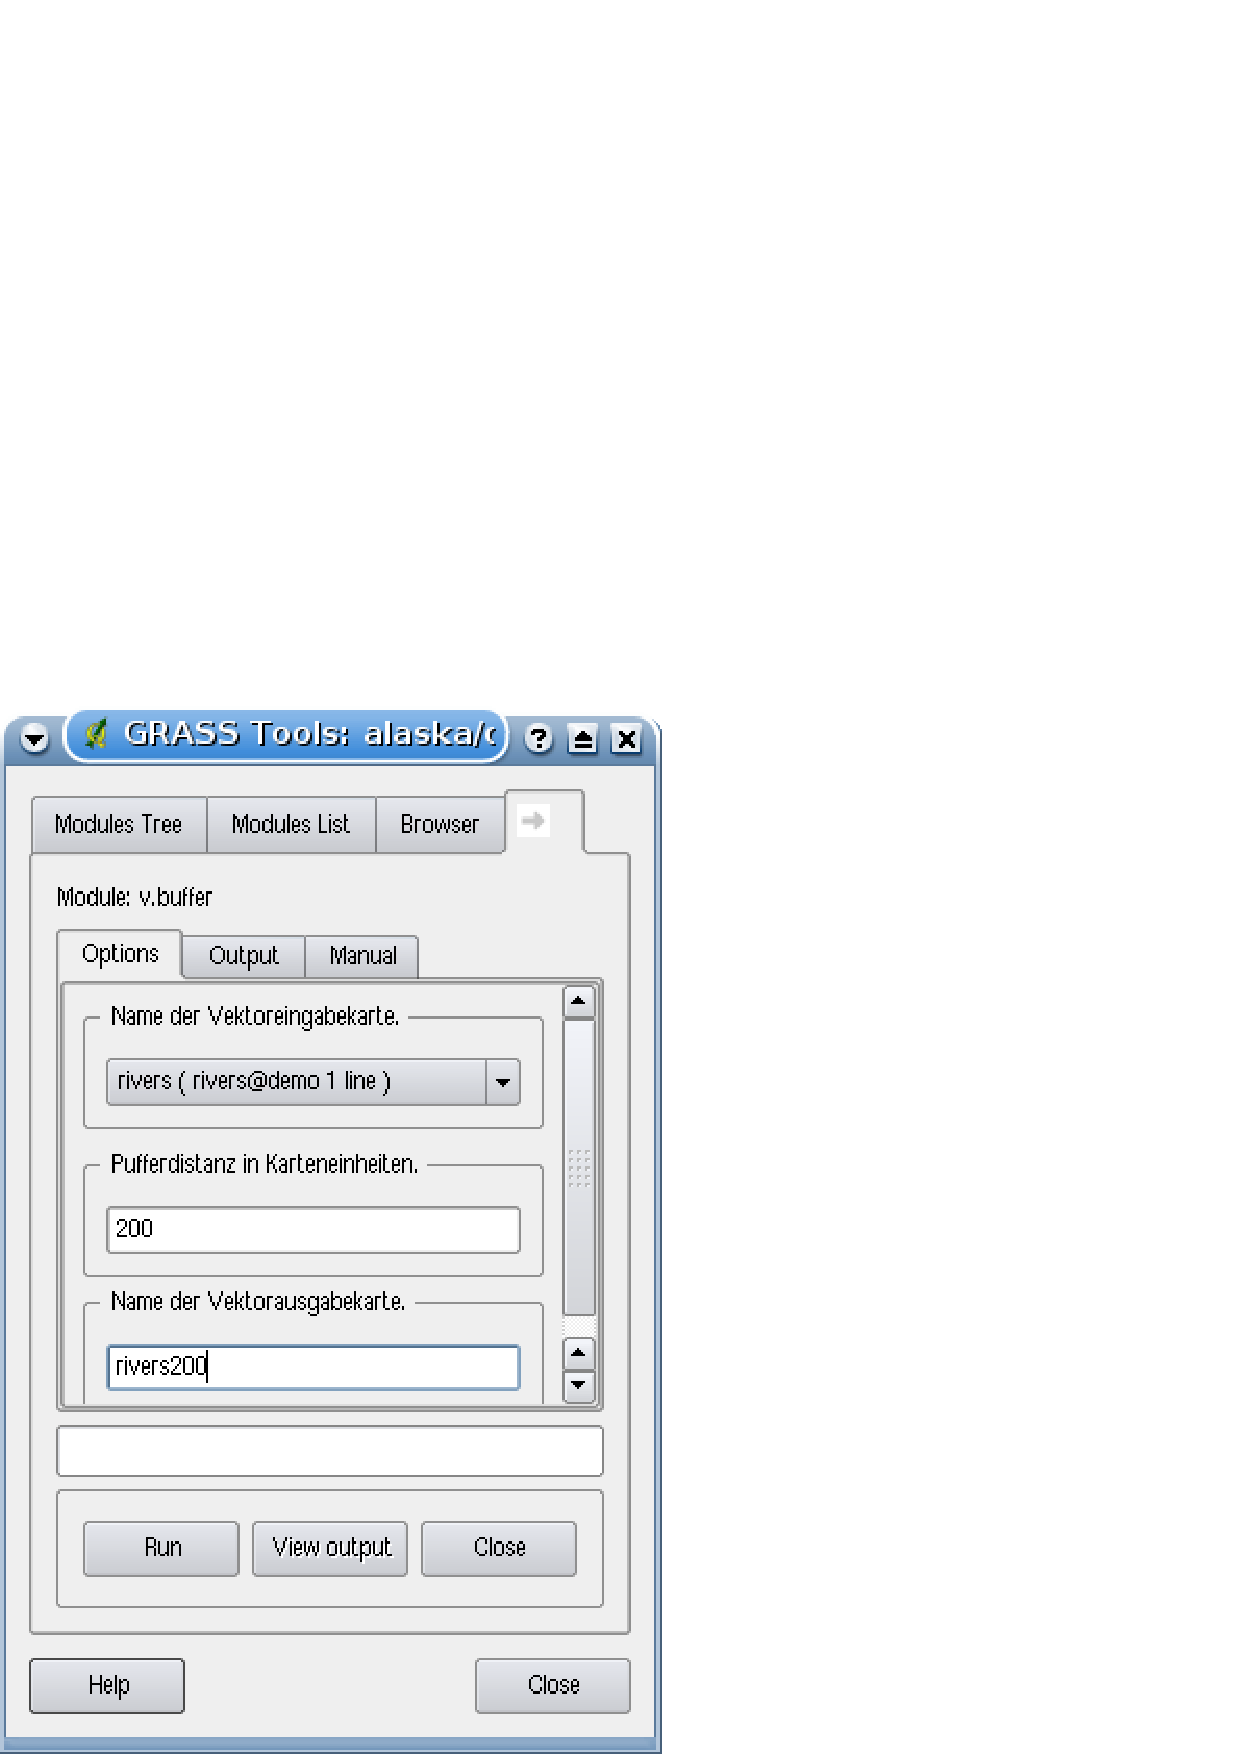
\includegraphics[clip=true, width=0.3\textwidth]{grass_module_option}}
   \hspace{1cm}
   \subfloat[Модули Вывод] {\label{subfig:grass_module_output}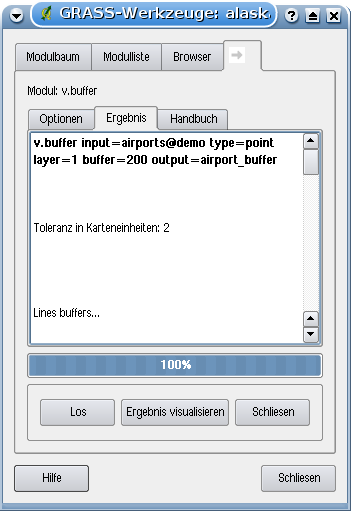
\includegraphics[clip=true, width=0.3\textwidth]{grass_module_output}}
   \hspace{1cm}
   \subfloat[Модули Справка] {\label{subfig:grass_module_manual}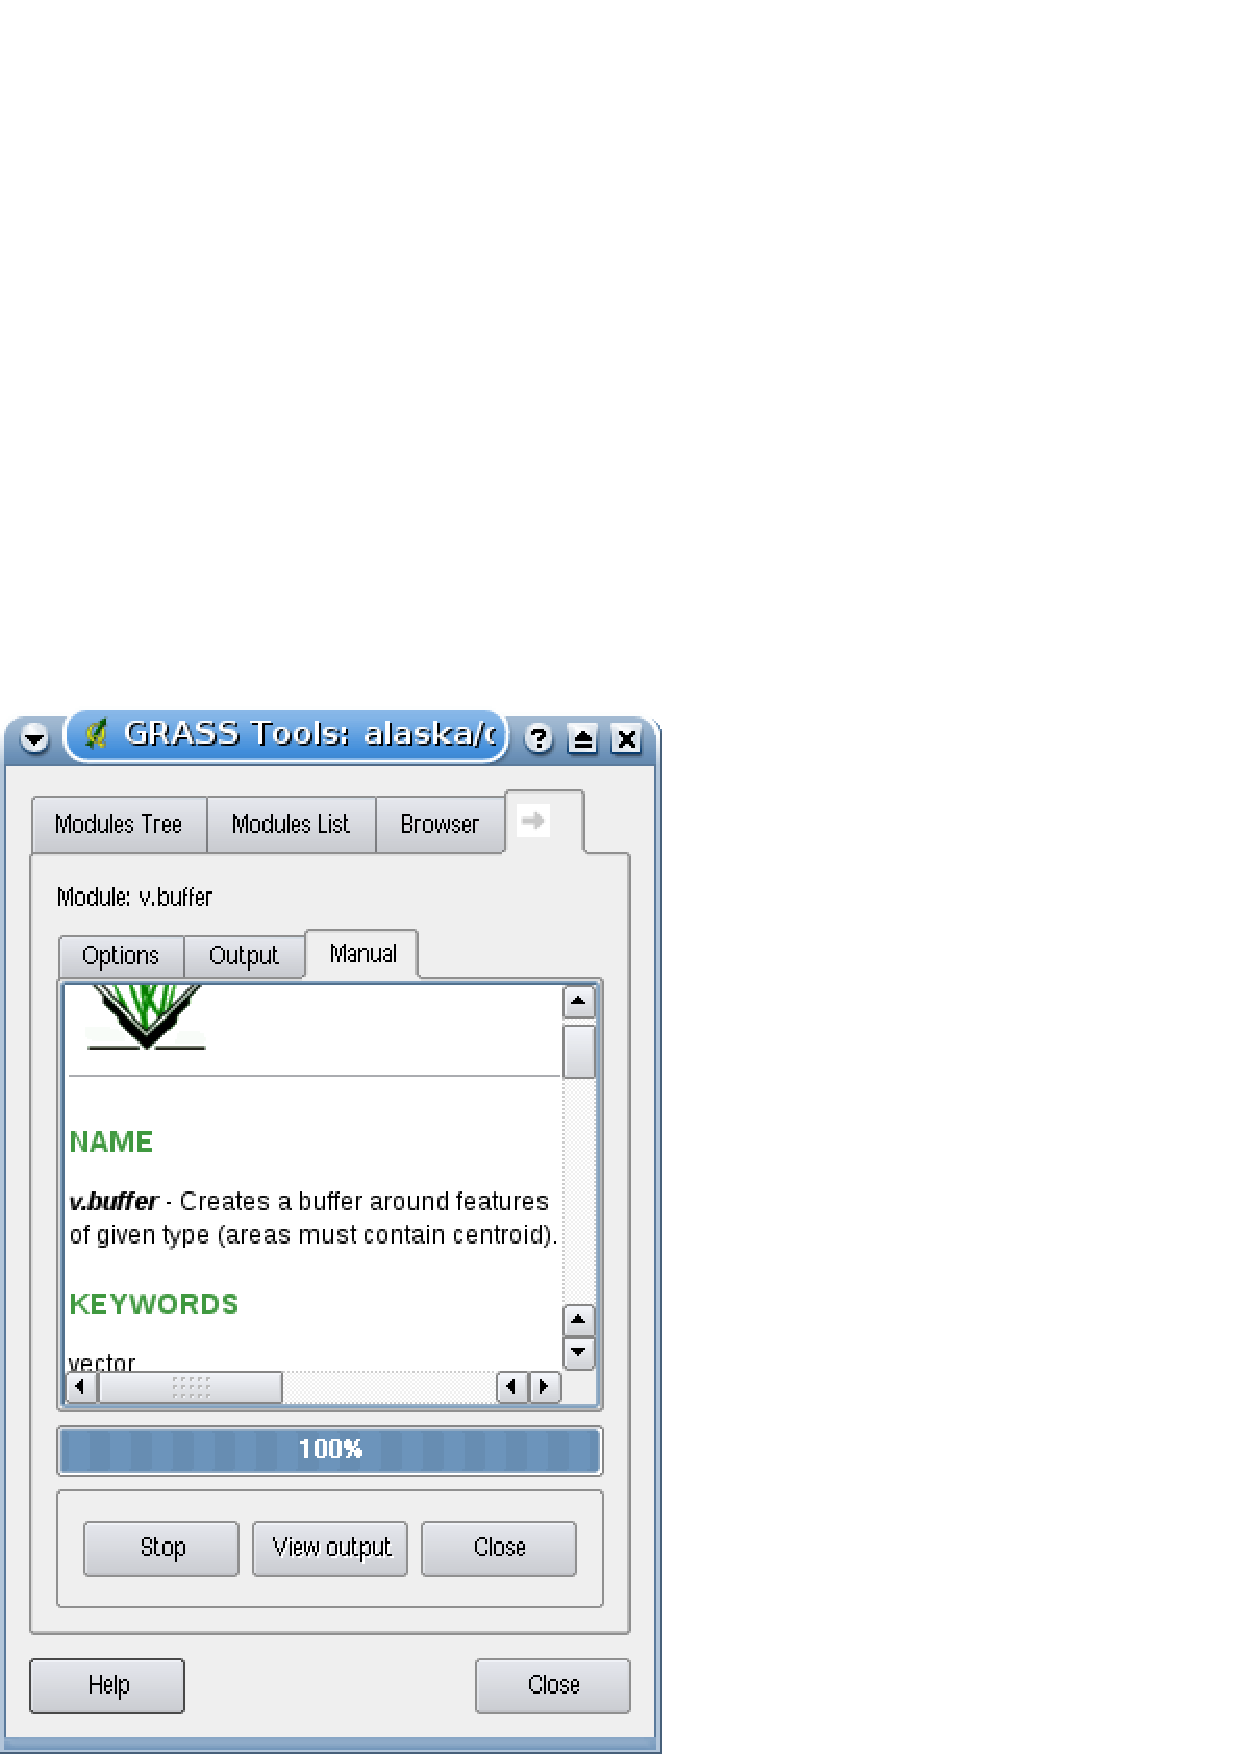
\includegraphics[clip=true, width=0.3\textwidth]{grass_module_manual}}
\caption{Диалоги модулей в инструментах GRASS \wincaption}\label{fig:grass_module_dialog}
\end{figure}
\FloatBarrier
\minisec{Параметры}

Вкладка \tab{Параметры} отображает упрощенный диалог модуля, где вы
можете обычно выбрать растровый или векторный слой, отображенный в окне
карты QGIS и ввести дальнейшие специфические параметры для запуска
модуля. Предоставляемые параметры модуля в большинстве случаев являются
неполным отражением диалога. Если вы хотите использовать остальные
параметры и флаги данного модуля, необходимо открыть оболочку GRASS и
запустить модуль из командной строки.

Новая функция в версии QGIS \CURRENT "--- поддержка кнопки
\button{Показать расширенные параметры >>} под упрощенным диалогом
модуля на вкладке \tab{Параметры}. В настоящее время эта функция
добавлена только для модуля v.in.ascii как образец, но, возможно, будет
добавлена для части модулей или всех модулей в будущих версиях QGIS.

\minisec{Вывод}

Вкладка \tab{Вывод} предоставляет информацию о статусе вывода модуля.
Когда вы нажимаете кнопку \button{Запустить}, модуль переключается во
вкладку \tab{Вывод} и вы можете видеть информацию о процессе анализа.
Если все закончилось успешно, в конце вы увидите сообщение
\usertext{Завершено успешно}.

\minisec{Справка}

Вкладка \tab{Справка} показывает HTML-страницу помощи по модулю GRASS.
Вы можете использовать ее для проверки дополнительных параметров модулей
и флагов или для более глубокого изучения назначения модуля. В конце
каждой страницы-мануала показаны дополнительные ссылки на
\filename{Main Help index}, \filename{Thematic index} и
\filename{Full index}. Эти ссылки дают ту же информацию, что и при
использовании модуля \filename{g.manual}.

\begin{Tip}\caption{\textsc{Показать результат сразу}}\index{GRASS!отображение результата}
Если вы хотите отобразить результаты выших вычислений сразу же в окне
карты, используйте кнопку <<Показать вывод>> внизу вкладки модуля.
\end{Tip}

\subsection{Примеры модулей GRASS}\index{GRASS!панель инструментов}

Следующие примеры продемонстрируют применение некоторых из модулей GRASS.

\minisec{Создание изолиний}

В первом примере создадим векторный слой изолиний из растровой карты
поверхности (цифровой модели рельефа). Предполагается, что вы имеете
\filename{Регион} Alaska, созданный так, как объяснено в разделе~
\ref{sec:import_loc_data}.

\begin{itemize}[label=--]
\item Сперва откройте область, нажав на кнопку
\toolbtntwo{grass_open_mapset}{Открыть набор} и выбрав область Alaska.
\item Теперь откройте карту рельефа \usertext{gtopo30}, нажав кнопку
\toolbtntwo{grass_add_raster}{Добавить растровый слой GRASS} и
выбрав растр \usertext{gtopo30} из набора demo.
\item Теперь откройте панель инструментов с помощью кнопки
\toolbtntwo{grass_tools}{Открыть инструменты GRASS}
\item В списке категорий инструментов выберите Растр -> Обработка
поверхностей -> Создание изолиний
\item Теперь единичный клик на инструменте \classname{r.contour}
откроет диалог, как было объяснено выше в разделе~\ref{grass_modules}.
Растр \usertext{gtopo30} должен появиться как
\inputtext{{}Имя исходной растровой карты}{gtopo30}.
\item Напечатайте в \inputtext{{}Шаг горизонталей}{100}
значение 100. (Тогда будут создаваться изолинии с интервалом в
100~метров).
\item Введите в \inputtext{{}Имя выходного векторного слоя}{ctour\_100}
имя \usertext{ctour\_100}.
\item Нажмите кнопку \button{Выполнить} для начала процесса. Подождите
некоторое время, пока в окне вывода не появится сообщение
\usertext{Успешное завершение}. Тогда нажмите кнопку
\button{Открыть вывод} и кнопку \button{Закрыть}.
\end{itemize}

\begin{figure}[ht]
\centering
   \subfloat[Параметры модуля r.contour] {\label{subfig:grass_toolbox_rcontour}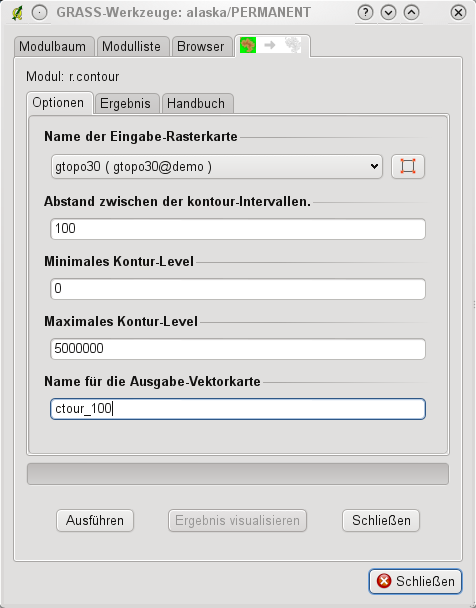
\includegraphics[clip=true, width=0.4\textwidth]{grass_toolbox_rcontour}}
    \hspace{0.5cm}
   \subfloat[Вывод модуля r.contour] {\label{subfig:grass_toolbox_rcontour2}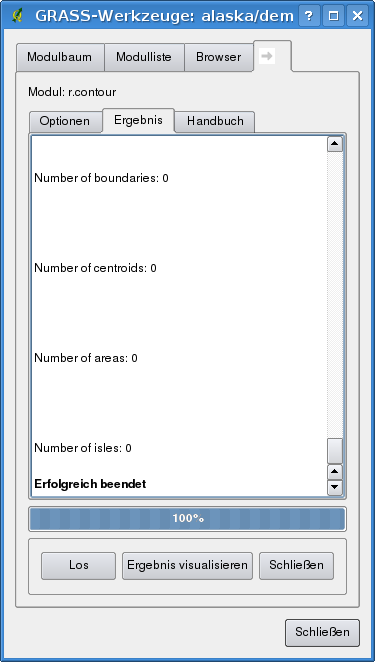
\includegraphics[clip=true, width=0.4\textwidth]{grass_toolbox_rcontour2}}
   \caption{\grass Инструменты GRASS, модуль r.contour \wincaption}\label{fig:grass_toolbox_rcontour}
\end{figure}


Так как текущий регион довольно обширен, отображение на экране может
занять какое-то время. После завершения отрисовки вы можете открыть окно
свойств слоя, чтобы изменить цвет линии, так, чтобы изолинии были заметны
на слое рельефа, как описано в разделе~\ref{sec:vectorprops}.

Следующим шагом увеличьте небольшой горный участок в центре Аляски.
Увеличив сильно, вы заметите, что изолинии имеют острые края. GRASS
предлагает инструмент \classname{v.generalize} для небольшого
видоизменения векторных карт с сохранением их общей формы. Инструмент
использует несколько различных алгоритмов для различных целей. Некоторые
из алгоритмов (например, Дугласа--Пойкера (Douglas--Peuker) и сокращения
узлов) упрощают линию путем удаления некоторой части вершин. Конечный
векторный слой будет подгружаться быстрее. Этот процесс может быть
использован, когда вы имеете очень подробную векторную карту, но
создаете мелкомасштабную карту, так что детали нежелательны.

\begin{Tip}\caption{\textsc{Инструмент упрощения геометрии}}\index{GRASS!отображение результата}
Заметьте, что модуль QGIS fTools имеет инструмент
\dropmenuopt{Упростить геометрию}, который работает почти так же, как алгоритм
Дугласа--Пойкера в \classname{v.generalize}.
\end{Tip}

Однако, цель этого примера другая. Изолинии, созданные модулем
r.contour, имеют острые края, которые должны быть сглажены. Среди
алгоритмов модуля \classname{v.generalize} имеется алгоритм Чейкена
(Chaikens), который как раз это делает (а также интерполяция кубическими
сплайнами Эрмитова (Hermite)). Имейте в виду, что эти алгоритмы могут и
\textbf{добавлять} дополнительные вершины к векторным объектам, что
может привести к их более медленной загрузке.

\begin{itemize}[label=--]
\item Откройте Инструменты GRASS и выберите Вектор -> Обработка карт ->
Генерализация, затем нажмите на модуль \classname{v.generalize}, чтобы
открыть окно его параметров.
\item Проверьте, что в графе
\inputtext{{}Имя исходного векторного слоя}{ctour\_100} находится
вектор \usertext{ctour\_100}.
\item Из списка алгоритмов выберите <<Алгоритм Чейкена>>. Оставьте
другие опции по умолчанию и промотайте вниз до последней строки, чтобы
ввести \inputtext{{}Имя выходного векторного слоя}{ctour\_100\_smooth},
и нажмите \button{Выполнить}.
\item Процесс займет какое-то время. Когда в окне вывода появится
сообщение \usertext{Успешное завершение}, нажмите \button{Открыть вывод}
и затем \button{Закрыть}.
\item Вы можете изменить цвет векторных изолиний, чтобы четче отобразить
их поверх растра и в контрасте с оригинальными изолиниями. Вы заметите,
что новые изолинии имеют более гладкие края, чем оригинальные, оставаясь
в целом исходной формы.
\end{itemize}

\begin{figure}[h]
 \centering
 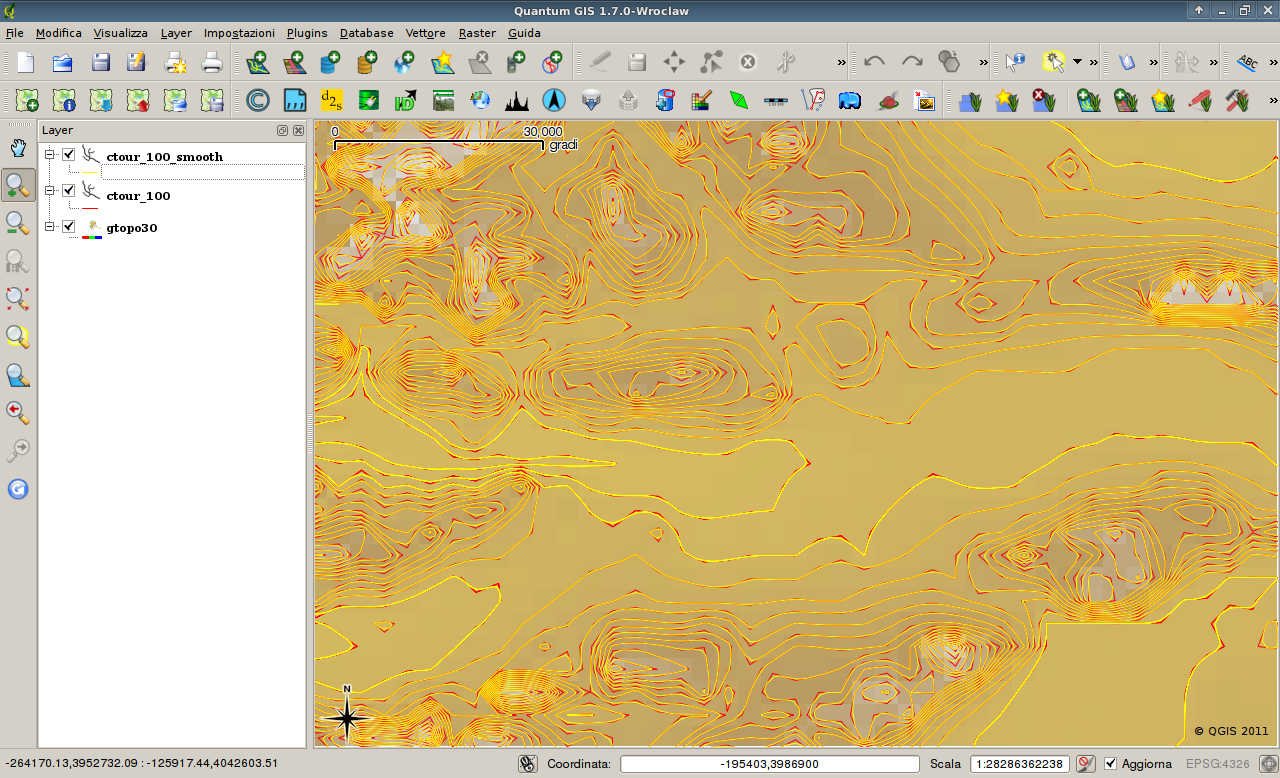
\includegraphics[clip=true, width=14cm]{grass_toolbox_vgeneralize}
 \caption{Модуль GRASS v.generalize для сглаживания объектов векторного слоя \wincaption}\label{fig:grass_toolbox_vgeneralize}
\end{figure}

\begin{Tip}\caption{\textsc{Другие применения модуля r.contour}}\index{GRASS!панель инструментов}

Процедура, описанная выше, может быть использована в других похожих
ситуациях. Например, если у вам есть растровая карта данных осадков, то
этот же способ может использоваться для создания векторной карты изогиет
(линий одинакового количества осадков).
\end{Tip}

\minisec{Создание 3D эффекта методом свето-теневой отмывки}

Для отображения земной поверхности и придания картам эффекта
трехмерности применяются несколько методов. Использование изолиний, как
показано выше, "--- один из популярных методов, часто применяемый при
производстве топографических карт. Другой метод получения 3D эффекта "---
с помощью т.\,н. свето-теневой отмывки. Свето-теневой эффект создается
на основе цифровой модели рельефа (ЦМР) сперва путём вычисления уклона
и экспозиции склонов в каждой ячейке, затем симуляцией позиции Солнца на
небосклоне и заданием значения отражения в каждой ячейке. Так вы
получаете освещенные склоны, находящиеся на пути света, и затемнённые,
находящиеся против света.

\begin{itemize}[label=--]
\item Начнем этот пример с загрузки карты поверхности \usertext{gtopo30}.
Запустите панель инструментов GRASS и в разделе Растр нажмите
Пространственный анализ -> Морфометрический анализ.
\item Затем выберите \classname{r.shaded.relief}, чтобы открыть этот
модуль.
\item Измените \inputtext{{}Азимут}{270} на 315. Введите
\usertext{gtopo30\_shade} для нового растра теневой отмывки и нажмите
\button{Выполнить}.
\item Когда процесс закончится, добавьте растр отмывки на карту. Как вы
видите, он отображается в серой цветовой шкале.
\item Чтобы увидеть вместе и теневую отмывку, и цвета \usertext{gtopo30},
передвиньте растр отмывки под растр \usertext{gtopo30} в слоях карты,
затем откройте окно \dropmenuopt{Свойства} слоя \usertext{gtopo30},
перейдите на вкладку \tab{Прозрачность} и выставите уровень
прозрачности 25\%.
\end{itemize}

Вы должны получить слой рельефа \usertext{gtopo30} с его цветовой
картой и заданной прозрачностью \textbf{поверх} слоя отмывки в серых
тонах. Для того, чтобы оценить визуальный эффект теневой отмывки
рельефа, отключите слой \usertext{gtopo30\_shade}, затем опять верните
его.

\minisec{Использование оболочки GRASS}

Расширение GRASS в QGIS разработано для пользователей, которые являются
новичками в GRASS, и не знакомы со всеми модулями и их опциями. Некоторые
модули, как таковые, не отображают на панели инструментов все возможные
параметры, а некоторые модули вообще не присутствуют. Оболочка GRASS (или
консоль) дает пользователю доступ к тем дополнительным модулям, которых
нет в дереве модулей, а также к некоторым дополнительным опциям тех
модулей, которые присутствуют на панели инструментов с минимальным
параметрами по умолчанию. Этот пример демонстрирует использование
расширенных опций в модуле \classname{r.shaded.relief}, который был
рассмотрен выше.

\begin{figure}[ht]
 \centering
 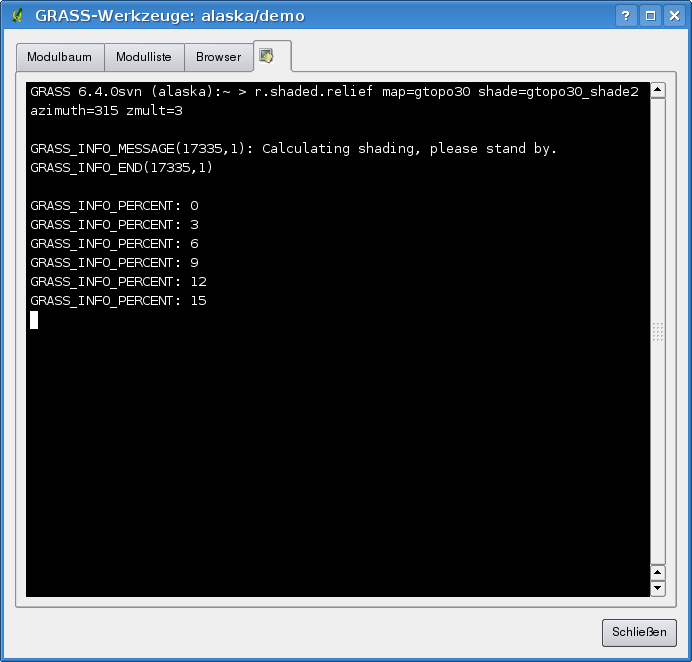
\includegraphics[clip=true, width=12cm]{grass_toolbox_shell}
 \caption{Оболочка GRASS, модуль r.shaded.relief \wincaption}\label{fig:grass_toolbox_shell}
\end{figure}

Модуль \classname{r.shaded.relief} может принимать параметр
\usertext{zmult}, который увеличивает значения поверхности относительно
единиц измерения координат X-Y так, что эффект теневой отмывки становится
более отчетливым.

\begin{itemize}[label=--]
\item Откройте карту рельефа \usertext{gtopo30} как сказано выше,
затем запустите Инструменты GRASS и выберите оболочку GRASS. В окне
оболочки введите команду:\linebreak
\usertext{r.shaded.relief map=gtopo30 shade=gtopo30\_shade2 azimuth=315
zmult=3} \linebreak и нажмите \keystroke{Enter}.
\end{itemize}

\begin{itemize}[label=--]
\item Когда процесс закончится, переключитесь на вкладку \tab{Браузер}
и дважды кликните на новом растре \usertext{gtopo30\_shade2}, чтобы
отобразить его в QGIS.
\item Как объяснено выше, переместите слой теневого рельефа ниже слоя
gtopo30 в списке слоев, затем проверьте прозрачность цветного растра
gtopo30. Вы должны увидеть, что 3D эффект усилился по сравнению с
первой картой теневой отмывки рельефа.
\end{itemize}

\begin{figure}[ht]
 \centering
 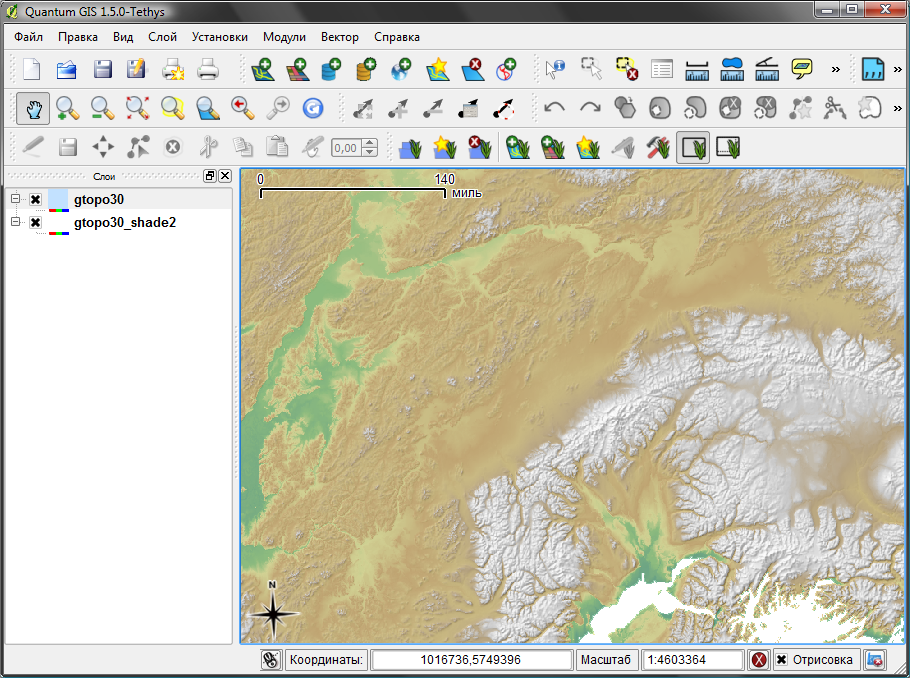
\includegraphics[clip=true, width=12cm]{grass_toolbox_shadedrelief}
 \caption{Карта теневой отмывки рельефа, созданная с помощью модуля
   r.shaded.relief \wincaption}\label{fig:grass_toolbox_shadedrelief}
\end{figure}

\minisec{Растровая статистика на векторной карте}

Следующий пример показывает, как модуль GRASS может обрабатывать
растровые данные и добавлять колонки статистики для каждого полигона в
векторном слое.

\begin{itemize}[label=--]
\item Снова используем данные набора данных Alaska, ссылаясь на
\ref{sec:import_loc_data} для импорта shape-файла растительности из
директории \usertext{vmap0\_shapefiles} в GRASS.
\item Теперь необходим промежуточный шаг: к импортированной карте
растительности нужно добавить центроиды, чтобы получить законченные
полигоны GRASS (включая и границы, и центроиды).
\item Из панели инструментов выберите Вектор -> Обработка объектов и
откройте модуль \classname{v.centroids}.
\item Введите \inputtext{{}Имя выходного векторного слоя}{\usertext{forest\_areas}}
и запустите модуль.
\item Теперь загрузите векторный слой \usertext{forest\_areas} и
отобразите типы лесов "--- лиственные, вечнозелёные, смешанные "--- в
различных цветах: в окне \dropmenuopt{Свойства}, вкладке
\tab{Символика}, выберите \\
\selectstring{{}Тип легенды}{Уникальное значения} и задать
\inputtext{{}Поле классификации}{VEGDESC}. (Обратитесь для
объяснения вкладки символики к секции~\ref{sec:symbology} в разделе
Вектор.
\item Далее заново откройте панель инструментов GRASS и выберите
Вектор -> Обновление данных на основе других карт.
\item Выберите модуль \classname{v.rast.stats}. Введите
\usertext{gtopo30} и \usertext{forest\_areas}.
\item Только один дополнительный параметр необходим: введите
\inputtext{{}column prefix}{\usertext{elev}} и нажмите \\
\button{Выполнить}. Это сложная вычислительная операция, которая будет
продолжаться долгое время (возможно, вплоть до двух часов).
\item Наконец, откройте таблицу атрибутов \usertext{forest\_areas} и
проверьте, что было добавлено несколько новых полей, включая
\usertext{elev\_min}, \usertext{elev\_max}, \usertext{elev\_mean} и
т.\,д. для каждого полигона в слое.
\end{itemize}

\subsection{Работа с браузером GRASS} \index{GRASS!панель инструментов!браузер}

Другой полезной функцией в Инструментах GRASS является браузер
\filename{Региона} GRASS. На рисунке~\ref{fig:grass_mapset_browser} вы
можете видеть текущий рабочий \filename{Регион} с его
\filename{Наборами}.

В левом окне браузера вы можете просматривать все \filename{Наборы}
внутри текущей \filename{Области}. В правом окне браузера показывается
некоторые метаданные для выбранных растровых или векторных слоев
(разрешение, охват, источник данных, присоединенная атрибутивная
таблица для векторных данных и история команд).

\begin{figure}[h]
 \centering
 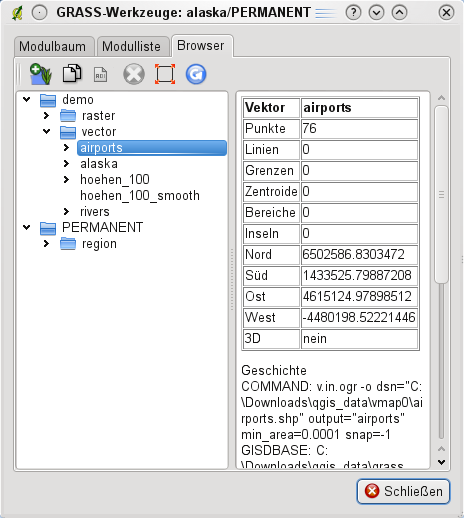
\includegraphics[clip=true,width=10cm]{grass_mapset_browser}
 \caption{Браузер GRASS \wincaption}\label{fig:grass_mapset_browser}
\end{figure}

Панель внутри вкладки \tab{Браузер} предлагает следующие инструменты
управления выбранной \filename{Областью}:

\begin{itemize}[label=--]
\item \toolboxtwo{grass_add_map}{{}Добавить выбранную карту в область QGIS}
\item \toolboxtwo{grass_copy_map}{{}Копировать выбранную карту}
\item \toolboxtwo{grass_rename_map}{{}Переименовать выбранную карту}
\item \toolboxtwo{grass_delete_map}{{}Удалить выбранную карту}
\item \toolboxtwo{grass_set_region}{{}Задать регион по границам выбранной
карты}
\item \toolboxtwo{grass_refresh}{{}Обновить}
\end{itemize}

Инструменты \toolboxtwo{grass_rename_map}{{}Переименовать выбранную карту}
и \toolboxtwo{grass_delete_map}{{}Удалить выбранную карту} работают только
с картами внутри текущего выбранного \filename{Набора}. Все остальные
инструменты работают также с растровыми и векторными слоями в других
\filename{Наборах}.


\subsection{Настройка инструментов GRASS} \index{GRASS!панель инструментов!настройка}
\label{sec:toolbox-customizing}

Практически все модули GRASS могут быть добавлены в панель инструментов
GRASS. Интерфейс XML производит анализ простых XML-файлов, которые
настраивают внешний вид и параметры модулей внутри панели инструментов.

Простой XML-файл для генерации модуля \usertext{v.buffer}
(v.buffer.qgm) выглядит примерно так:
\begin{verbatim}
<?xml version="1.0" encoding="UTF-8"?>
<!DOCTYPE qgisgrassmodule SYSTEM "http://mrcc.com/qgisgrassmodule.dtd">

<qgisgrassmodule label="Vector buffer" module="v.buffer">
        <option key="input" typeoption="type" layeroption="layer" />
        <option key="buffer"/>
        <option key="output" />
</qgisgrassmodule>
\end{verbatim}

Парсер читает это описание и создает новую вкладку внутри панели
инструментов при выборе модуля. Более детальное описание добавления
новых модулей, изменения групп модулей и т.\,д. может быть найдено на
QGIS Wiki по адресу \\
\url{http://wiki.qgis.org/qgiswiki/Adding\_New\_Tools\_to\_the\_GRASS\_Toolbox}.

\FloatBarrier
